\documentclass{sig-alternate}



% SOME OF OUR DEFINITIONS

\usepackage{xspace}
\newcommand{\sys}{MBArk\xspace}
%\newcommand{\sys}{Embark\xspace}
%\newcommand{\sys}{EMBArk\xspace}
\newcommand{\RM}{RM\xspace}
% MBArk
% EMBArk

\usepackage{fancyvrb}
\usepackage{listings}



\lstset{
  basicstyle=\footnotesize\ttfamily, 
  columns=fullflexible,
  keepspaces=true,
}

\usepackage{subfigure}
\usepackage{ifpdf}
\usepackage[usenames,dvipsnames]{color}
\usepackage[letterpaper, breaklinks, pdfborder={0 0 0}]{hyperref}
\hypersetup{
  backref=true
  bookmarksnumbered,
  colorlinks=true,
  pdfstartview={FitH},
  citecolor={blue},
  linkcolor={blue},
  urlcolor={blue},
  citecolor={blue},
  pdfpagemode={UseOutlines}
  }
  
  %\usepackage{algorithmic}
  
\usepackage[noend]{algpseudocode}

% edit the comments 
\usepackage{eqparbox}
\renewcommand{\algorithmiccomment}[1]{\eqparbox{COMMENT}{// {\emph #1}}}
  
%\usepackage{multicol}
%\usepackage{amsmath, amssymb}
%\usepackage{amsthm}
\usepackage{enumitem}
%\usepackage{rotating}
%\onehalfspacing
%\newcommand{\tbd}[1]{[{\bf{#1}}]}
\newcommand{\tbd}[1]{}
\newcommand{\ie}{{\it i.e.}}
\newcommand{\eg}{{\it e.g.}}
\newcommand{\etc}{{\it etc.}}
\newcommand{\eat}[1]{}


\newcommand{\mypara}[1]{\medskip\noindent{\bf {#1}.}~}
\newcommand{\submypara}[1]{\medskip\noindent{\it {#1}.}~}
\newcommand{\chk}{$\checkmark$}
\newcommand{\dsh}{{\bf --}}
\newcommand{\til}{{\bf\large \textasciitilde}}
\usepackage{rotating}

\usepackage{framed}

\newcommand{\CTE}{CTE\xspace}
\newcommand{\Name}{APLOMB\xspace}
\newcommand{\Nameplus}{{APLOMB+}\xspace}
\newcommand{\NameArch}{{\sc APLOMB}\xspace}

% RESULTS

\newcommand{\generalFHEslowdown}{9\xspace}
\newcommand{\squaregeneralFHEslowdown}{18}
\newcommand{\strawmanslowdown}{10^6}
\newcommand{\setuptime}{414 s}
\newcommand{\strawmansetuptimesslower}{1.8 \cdot 10^3}

\usepackage{enumitem}
\setlist[itemize]{itemsep=0.00cm}
\setlist[itemize]{parsep=0.01cm}
%\setlist[itemize]{parskip=0.01cm}


\newenvironment{myitemize}
{ \begin{itemize}[nolistsep]
    \setlength{\itemsep}{0.5pt}
    \setlength{\parskip}{0.9pt}
    \setlength{\parsep}{0.1pt}     }
{ \end{itemize}                  } 

\newcommand{\simplequote}[1]{\\\noindent{\it``{#1}''}\linebreak[3]}
\newcommand{\green}[1]{{\color{ForestGreen}{#1}}}


% our encryption scheme
\newcommand{\bbenc}{DPIEnc\xspace}
\newcommand{\bbdetect}{\sys Detect\xspace}

\newcommand{\RG}{RG\xspace}
\newcommand{\MB}{MB\xspace}

\newcommand{\sslk}{k_{\mathsf{SSL}}}
\newcommand{\bbG}{\mathbb{G}}

\newcommand{\garble}{\mathsf{Garble}}
\newcommand{\eval}{\mathsf{Eval}}
\newcommand{\keygen}{\mathsf{KeyGen}}
\newcommand{\Enc}{\mathsf{Enc}}
\newcommand{\kwenc}{\mathsf{KWEnc}}
\newcommand{\enc}{\Enc}
\newcommand{\en}{\mathsf{enc}}
\newcommand{\encleft}{\mathsf{EncLeft}}
\newcommand{\encright}{\mathsf{EncRight}}
\newcommand{\match}{\mathsf{Match}}

\newcommand{\sig}{\mathsf{sig}}
\newcommand{\ct}{\mathsf{ct}}
\newcommand{\sno}{\mathsf{serial\_no}}

\renewcommand{\mod}{\mathsf{mod}\xspace}

\newcommand{\low}{\mathsf{low}\xspace}
\newcommand{\high}{\mathsf{high}\xspace}
\newcommand{\prf}{\mathsf{prf}\xspace}

\newcommand{\twosnortcom}{67\%}
\newcommand{\twosnortemerge}{42\%}


\newcommand{\SSL}{\mathsf{SSL}}
\newcommand{\rand}{\mathsf{rand}}
\newcommand{\salt}{\mathsf{salt}}
% requires amsthm, enumitem                                                                        
%\theoremstyle{algorithms}
%\newtheorem{construction}{Algorithm}
%\newcommand{\ALGORITHM}[4]{%  name, llabel, intro, \items                                          
%\begin{construction}[#1]\label{#2} \mbox{}
%\normalfont\noindent
% #3
% \vspace{0.13\baselineskip}
% \begin{enumerate}[noitemsep,nolistsep]\itemsep=0.1\baselineskip
% #4
% \end{enumerate}
% \end{construction}
%}



\newcommand{\ALGORITHM}[4]{%  name, llabel, intro, \items    
\let\oldi\labelenumi
\let\oldii\labelenumii
\let\oldiii\labelenumiii
\renewcommand{\labelenumi}{\arabic{enumi}: }
\renewcommand{\labelenumii}{\arabic{enumi}.\arabic{enumii}: }
\renewcommand{\labelenumiii}{\arabic{enumi}.\arabic{enumii}.\arabic{enumiii}: }                                     
\noindent \textbf{#1:} \label{#2} 
#3
 \vspace{0.13\baselineskip}
 \begin{enumerate}[noitemsep,nolistsep]\itemsep=0.1\baselineskip
 #4
 \end{enumerate}
 \let\labelenumi\oldi
\let\labelenumii\oldii
\let\labelenumiii\oldii  
}

\newcommand{\subparagraph}{\paragraph}
\usepackage[compact]{titlesec}

%\newcommand{\simplequote}[1]{\begin{quote}{\it{#1}}\end{quote}}

%\renewcommand\%bibname{}


%\usepackage[compact]{titlesec}  
%\titlespacing{\section}{0pt}{0pt}{0pt}
%\titlespacing*{?command?}{?left?}{?beforesep?}{?aftersep?}[?right?]



\newcommand{\tickYes}{\checkmark}
\newcommand{\todo}[1]{{\color{Red} [todo: {#1}]}}
\newcommand{\justine}[1]{{\color{Red} JS: {#1}}}
\newcommand{\raluca}[1]{{\color{Red} RP: {#1}}}
\newcommand{\clan}[1]{{\color{Red} CL: {#1}}}
\newcommand{\sr}[1]{{\color{CarnationPink} SR: {#1}}} % :)
\newcommand{\shaddi}[1]{{\color{SkyBlue} SH: {#1}}} % :)
\newcommand{\qu}[1]{{\color{Magenta}  {\bf Question:} {#1}}} 
\newcommand{\warning}[1]{{\color{Red}{\bf Warning: #1}}}

\newcommand{\aes}{\mathsf{AES}}
\newcommand{\encr}{\mathsf{enc\_r}}

\begin{document}



%
% --- Author Metadata here ---
%\conferenceinfo{WOODSTOCK}{'97 El Paso, Texas USA}
%\CopyrightYear{2007} % Allows default copyright year (20XX) to be over-ridden - IF NEED BE.
%\crdata{0-12345-67-8/90/01}  % Allows default copyright data (0-89791-88-6/97/05) to be over-ridden - IF NEED BE.
% --- End of Author Metadata ---

\title{\sys: Securely outsourcing middleboxes to the cloud \\ {\small \qu{should we call the system Embark?}}}

\subtitle{Paper ID: \#??}


%
% You need the command \numberofauthors to handle the 'placement
% and alignment' of the authors beneath the title.
%
% For aesthetic reasons, we recommend 'three authors at a time'
% i.e. three 'name/affiliation blocks' be placed beneath the title.
%
% NOTE: You are NOT restricted in how many 'rows' of
% "name/affiliations" may appear. We just ask that you restrict
% the number of 'columns' to three.
%
% Because of the available 'opening page real-estate'
% we ask you to refrain from putting more than six authors
% (two rows with three columns) beneath the article title.
% More than six makes the first-page appear very cluttered indeed.
%
% Use the \alignauthor commands to handle the names
% and affiliations for an 'aesthetic maximum' of six authors.
% Add names, affiliations, addresses for
% the seventh etc. author(s) as the argument for the
% \additionalauthors command.
% These 'additional authors' will be output/set for you
% without further effort on your part as the last section in
% the body of your article BEFORE References or any Appendices.

\numberofauthors{8} %  in this sample file, there are a *total*
% of EIGHT authors. SIX appear on the 'first-page' (for formatting
% reasons) and the remaining two appear in the \additionalauthors section.
%
\author{
% You can go ahead and credit any number of authors here,
% e.g. one 'row of three' or two rows (consisting of one row of three
% and a second row of one, two or three).
%
% The command \alignauthor (no curly braces needed) should
% precede each author name, affiliation/snail-mail address and
% e-mail address. Additionally, tag each line of
% affiliation/address with \affaddr, and tag the
% e-mail address with \email.
%
% 1st. author
%\alignauthor
%Ben Trovato\titlenote{Dr.~Trovato insisted his name be first.}\\
%       \affaddr{Institute for Clarity in Documentation}\\
%       \affaddr{1932 Wallamaloo Lane}\\
%       \affaddr{Wallamaloo, New Zealand}\\
%       \email{trovato@corporation.com}
% 2nd. author
%\alignauthor
%G.K.M. Tobin\titlenote{The secretary disavows
%any knowledge of this author's actions.}\\
%       \affaddr{Institute for Clarity in Documentation}\\
%       \affaddr{P.O. Box 1212}\\
%       \affaddr{Dublin, Ohio 43017-6221}\\
%       \email{webmaster@marysville-ohio.com}
%% 3rd. author
%\alignauthor Lars Th{\o}rv{\"a}ld\titlenote{This author is the
%one who did all the really hard work.}\\
%       \affaddr{The Th{\o}rv{\"a}ld Group}\\
%       \affaddr{1 Th{\o}rv{\"a}ld Circle}\\
%       \affaddr{Hekla, Iceland}\\
%       \email{larst@affiliation.org}
%\and  % use '\and' if you need 'another row' of author names
%% 4th. author
%\alignauthor Lawrence P. Leipuner\\
%       \affaddr{Brookhaven Laboratories}\\
%       \affaddr{Brookhaven National Lab}\\
%       \affaddr{P.O. Box 5000}\\
%       \email{lleipuner@researchlabs.org}
%% 5th. author
%\alignauthor Sean Fogarty\\
%       \affaddr{NASA Ames Research Center}\\
%       \affaddr{Moffett Field}\\
%       \affaddr{California 94035}\\
%       \email{fogartys@amesres.org}
%% 6th. author
%\alignauthor Charles Palmer\\
%       \affaddr{Palmer Research Laboratories}\\
%       \affaddr{8600 Datapoint Drive}\\
%       \affaddr{San Antonio, Texas 78229}\\
%       \email{cpalmer@prl.com}
}
% There's nothing stopping you putting the seventh, eighth, etc.
% author on the opening page (as the 'third row') but we ask,
% for aesthetic reasons that you place these 'additional authors'
% in the \additional authors block, viz.
%\additionalauthors{Additional authors: John Smith (The Th{\o}rv{\"a}ld Group,
%email: {\texttt{jsmith@affiliation.org}}) and Julius P.~Kumquat
%(The Kumquat Consortium, email: {\texttt{jpkumquat@consortium.net}}).}
\date{30 July 1999}
% Just remember to make sure that the TOTAL number of authors
% is the number that will appear on the first page PLUS the
% number that will appear in the \additionalauthors section.

\maketitle

%!TEX root = mb.tex

\begin{abstract}

Network middleboxes such as firewalls, NAT, proxies, and intrusion prevention systems are crucial components of modern networks. Recently, more and more organizations are outsourcing their middleboxes to the cloud. However, this poses a problem for the confidentiality of the traffic because now the cloud provider has access to the organization's traffic.


We design and build \sys (read ``embark''), the first system that enables running a wide range of middleboxes at a cloud provider while maintaining the confidentiality of traffic. \sys encrypts the traffic that reaches the cloud and enables the cloud to process the {\em encrypted} traffic without decrypting it.
\sys supports a wide-range of middleboxes such as firewall, NAT, web proxy, load balancing, IP forwarding, intrusion prevention systems, data exfiltration systems, and VPN. Our evaluation shows that \sys supports these applications with competitive performance: because \sys makes no modifications to the dataplane for most middleboxes, throughput at most middleboxes is uneffected by our changes.

\end{abstract}


% A category with the (minimum) three required fields
%\category{H.4}{Information Systems Applications}{Miscellaneous}
%A category including the fourth, optional field follows...
%\category{D.2.8}{Software Engineering}{Metrics}[complexity measures, performance measures]


%\terms{Systems}

%\keywords{ACM proceedings, \LaTeX, text tagging}

%!TEX root = mb.tex


\section{Introduction}\label{sec:intro}


    Network processing appliances (``middleboxes'') such as firewalls, NATs, proxies, and intrusion detection systems are crucial components of modern networks~\cite{aplomb}. 
    In recent trends, more and more organizations are {\it outsourcing} their network processing, either to cloud providers~\cite{aplomb, aryaka, zscalar} or to Internet service providers who refer to this trend as Network Functions Virtualization (NFV)~\cite{nfv}.
    This strategy promises to reduce costs, decrease the burden of managing and configuring these devices, and provide redundant resources for elasticity and fault tolerance~\cite{aplomb}.
    Already now, the NFV working group~\cite{nfvwg} has over 250 members ranging from large telecoms to hardware manufacturers, all of whom are investing in new technologies to enable outsourced traffic processing.
   
   Nevertheless, outsourcing middleboxes to a third party service provider brings a new and important challenge: the confidentiality of the traffic. In order to be able to process and examine the traffic of an organization, the cloud  receives  the traffic {\em unencrypted}.  This means that the cloud now has access to potentially sensitive packet payloads,  IP addresses, and ports revealing confidential information about the organization. This situation is worrisome considering the number of documented data breaches by cloud employees or hackers gaining access to clouds~\cite{PrivacyRecords}.
   Hence, an important question is: can we enable a third party to perform traffic processing for an enterprise, {\em without seeing the enterprise's traffic}?
   
   
   

% Justine's text unchanged: (the above is a combination of Justine & Raluca)
%    Network processing appliances (''middleboxes'') such as firewalls, proxies, and intrusion detection systems make up a substantial fraction of modern network infrastructure; studies show that as much as 1/3 of enterprise network hardware consists of such devices~\cite{aplomb}.
%    However, recent trends suggest that this fraction may begin to decline as more and more networks begin to {\it outsource} their network processing, either to cloud providers~\cite{aplomb, aryaka, zscalar} or to service providers through Network Functions Virtualization (NFV)~\cite{nfv}.
%    At the time of this writing, the NFV working group~\cite{nfvwg} has over 250 members ranging from large telecoms to hardware manufacturers, all of whom are investing in new technologies to enable outsourced traffic processing.
%    For consumers, outsourcing traffic processing offers many of the same benefits that outsourcing compute and storage have attained through cloud computing: decreased costs, ease of management, the ability to scale and failover on demand, \etc{}.
%    Nevertheless, outsourcing network processing brings new challenges, and among them, an issue which is critical to most enterprises: privacy.
%    
%    Under traditional middlebox deployments, traffic is processed and inspected by devices which are owned, hosted, and managed entirely within the enterprise itself.
%    Encrypted traffic is often decrypted to enable deep packet inspection (DPI) such as intrusion detection and exfiltration detection.
%    This configuration places critical trust in the hands of network administrators, who can potentially read or even modify {\it any} connection within the company.
%    Outsourcing shifts this trust away from network administrators who are employed and monitored by the company whose data is being processed, and to a third party company with its own employees, hiring practices, and motivations.
%    Hence, in this paper, we ask: is it possible to enable a third party to perform traffic processing for an enterprise, without transferring the ability to read and monitor the enterprise's traffic?
%    
% 
     
     
     
  
    We design and build \sys, the first system that enables running a wide range of middleboxes at a cloud  while maintaining the confidentiality of the traffic. \sys provides these guarantees even against attackers who gained access to {\em all} the data at the cloud.  \sys's name concatenates the words MB (middlebox) and Ark (protection). \sys supports a wide range of middleboxes, in fact, all middleboxes that~\cite{aplomb} documents to be fit for cloud outsourcing. We list these middleboxes in Table~\ref{tab:apps-ops}. Moreover, \sys supports these middleboxes with almost no penalty in typical middlebox throughput despite our changes. 
    
    The approach in \sys is to encrypt the traffic that goes to  the middleboxes in the cloud and enable the cloud to process encrypted traffic without ever decrypting it. \sys encrypts the packet payload as well as important information in the header (such as IP addresses and ports). Since the service provider receives only encrypted traffic and no decryption key, it cannot see the confidential data. However, designing a practical system that supports a wide-range of middlebox applications over encrypted traffic is challenging and required a set of new cryptographic and systems techniques.
    
    
\newcounter{theapp} \setcounter{theapp}{0}  
\newcommand{\capp}{\refstepcounter{theapp}\arabic{theapp}}
    
\begin{table}[t!]
\centering  
\begin{tabular}{c|p{3.3cm}|p{0.6cm}|p{2.5cm}}
& {\bf Middlebox}  & {\bf Type } & {\bf Example fields}  \\
\hline \hline
\capp &  IP Firewall \S\ref{sec:firewall} & HO &  IP address   \\
\capp &  Application Firewall  \S\ref{sec:firewall} & BA & IP address  \\
\capp & NAT  \S\ref{sec:nat} & HO & IP address  \\
\capp & IP Forwarding  \S\ref{sec:other_apps}  & HO &  IP address \\
\capp & Load Balancer L4 \S\ref{sec:loadb} & HO & IP address  \\
\capp & Load Balancer L7 \S\ref{sec:loadb} & BA & URL in payload  \\
\capp & Web Proxy/Cache  \S\ref{s:proxy} & HO & URL in payload \\
\capp & Intrusion Detect (IDS) \S\ref{sec:ids} & BA & payload \\
\capp & Data Exfiltration  \S\ref{sec:ids} & BA & payload \\
\capp & VPN Gateway \S\ref{sec:vpn} &  HO &  IP address \\ 
\end{tabular}
\caption{Middleboxes supported by \sys, shown with the section that discusses them, their type, HO (header only) or BA (bytestream aware), and one  example of an encrypted field  each operates on. \label{tab:apps-ops} }
\end{table}

% 2nd fig/1st fig = 1.12 ratio
\begin{figure*}[t!]
\centering
\hspace{.2in}
\subfigure[Enterprise to external site communication]{
  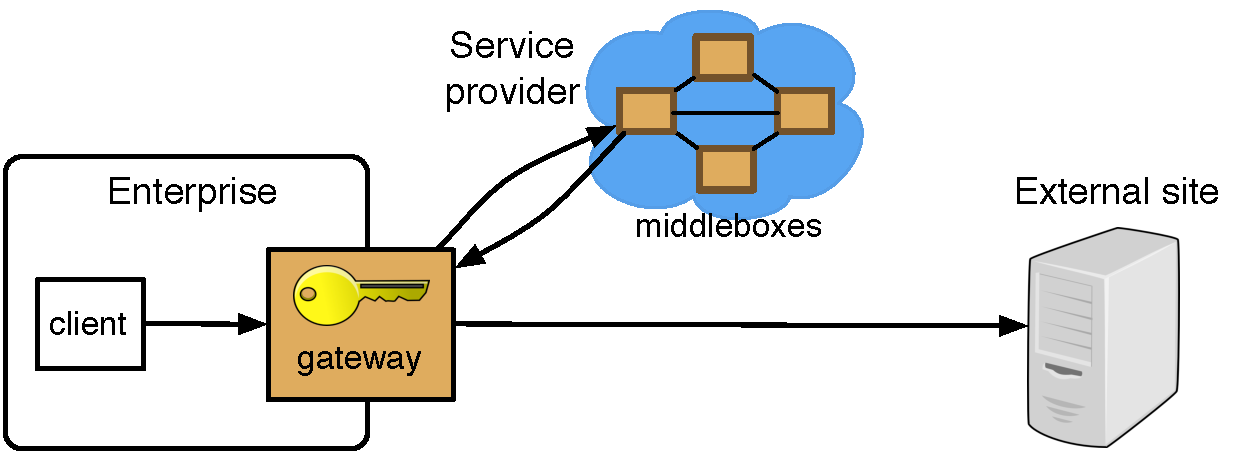
\includegraphics[width=2.5in]{fig/model_1.pdf}
  \label{fig:model1} }
%
\subfigure[Enterprise to enterprise communication]{
   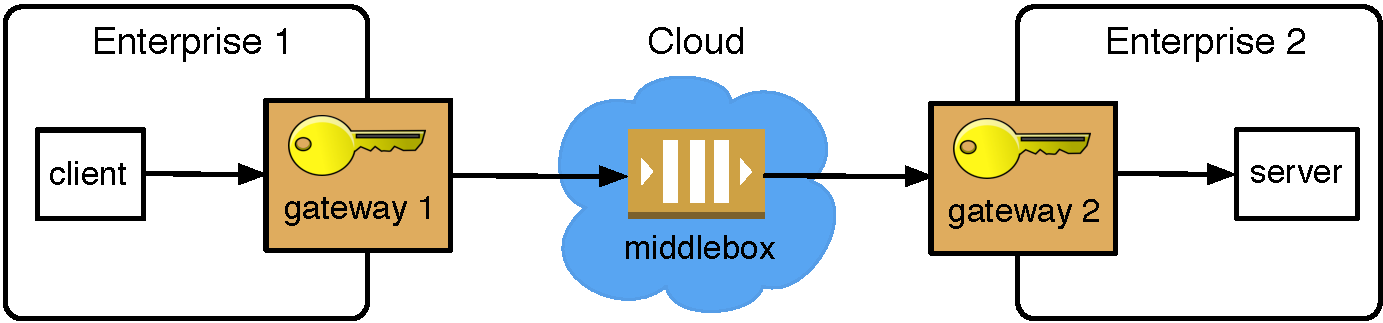
\includegraphics[width=3.0in]{fig/model_2.pdf}
     \label{fig:model2}}
     %
\caption{System architecture. Aplomb and NFV system setup with \sys encryption  at the gateway. The arrows indicate traffic from the client to the server; the response traffic follows the reverse direction. \label{fig:sys-overview}}
\end{figure*}


    
The first challenge is that performing generic computation on encrypted data is prohibitively impractical. The applications considered provide complex functionalities. For example, firewall and NAT examine packet header information such as IP addresses and ports; for IDS and data exfiltration detection, the middlebox (MB) examines the packet payload and tries to match complex rules (e.g., keywords, regular expressions). For each packet, a middlebox must process a packet on the timescale of microseconds. 

%Shrunk re: feedback that it was (a) too long, (b) too "chestbeaty" -- giving credit to CryptDB for the vision without sounding like we're bragging
Existing generic homomorphic encryption schemes are many orders of magnitude impractical~\cite{gentry:fhe-aes-eprint}, not just for middleboxes but for most systems (even those with more relaxed performance requirements).
This paper hence takes inspiration from CryptDB~\cite{popa:cryptdb}. Instead of using a generic encryption scheme, CryptDB proposes to identify core operations that underlie the functionality of the system and to support each with a specialized and fast encryption scheme. 
Unfortunately, CryptDB encrypts data operated on by a database; neither the encryption schemes nor the systems techniques in CryptDB meet the tight performance requirements of our network setting.

We identify two core operations that underlie middlebox processing: {\em keyword match} and {\em range match}. Keyword match refers to  identifying if a keyword appears in a byte stream.   For example, keyword match is useful for a web proxy: the service provider can identify if a filename cached at the proxy appears in a HTTP GET request in the packet flow. % data exfiltration when a watermark is searched for in the traffic, for IDS when malicious strings are searched for in the traffic and for web proxy for matching file identifiers that could be potentially in a cache. 
Range match enables determining if a value $x$ is in an interval [$x_1$, $x_2$], for example, if an IP address is in the range [18.0.0.0, 18.255.255.255] (\ie{} the prefix 18.0.0.0/8).
%\clan{people are familiar with longest prefix matching. maybe we should point out that prefix matching is strictly a special instance of range matching.} 
%An example middlebox that uses range match is the firewall. For example, the firewall has to determine if a source IP address from a packet falls in a certain range of IP addresses and, if so, apply a certain action to the packet.  
Note that range match supports a basic version of keyword match, namely complete equality check, when the range consists of only one value.
%
Table~\ref{tab:apps-ops} summarizes the middleboxes we support and the operations they rely on. 


% TO CUT/REMOVE: just say that they are too insecure and slow and don't explain about order
A second challenge is that, although there exist algorithms for keyword match, there is no suitable encryption scheme for the range match scheme:
 the only practical schemes applicable here perform order-preserving encryption (OPE)~\cite{boldyreva:ope,popa:mope}, and are both too insecure and too slow for our setting.  For example, OPE schemes leak the order of the values encrypted. We designed a new encryption scheme, called {\em RangeMatch}, which is targeted at and takes advantage of the network setting. RangeMatch  is fast (performing encryptions in under 3$\mu$s, 3 orders of magnitude faster than the OPE schemes) and it is more secure because it does not reveal the order of the values encrypted. 
 
A last challenge is to design and build a system that supports the variety of applications mentioned, is practical and easy to deploy. 
To address this challenge, we make the following contributions:

\noindent (a) We design a  protocol for each type of middlebox in Table~\ref{tab:apps-ops} by employing our two encrypted match  primitives.

\noindent (b) We integrate these protocols in a way that {\em does not change the existing packet structure}. We achieve this by ensuring that our encrypted values fit into the space of the unencrypted values, leverage the IPv6 options header, and sometimes add a second network flow.

\noindent (c) For most middleboxes, we keep {\em unchanged  the algorithms employed on the fast path} data plane which processes packets. In particular, firewalls implemented in hardware can use the existing hardware unchanged.  This enables middlebox throughput with \sys to almost match throughput without \sys, despite our changes.




We implemented and evaluated \sys on EC2. As mentioned, we support all applications that fit in the cloud outsourcing model, as surveyed in~\cite{aplomb} -- any appliance which is outsourced today can also be outsourced using \sys.
Further, \sys imposes negligible throughput overheads at the service provider: for example, a firewall operating over encrypted data achieves 9.8Gbps, equal to the same firewall over unencrypted data.
Our gateway can forward at 1.5 Gbps on a single core; our 8 core server can transmit \sys encrypted data at up to 8Gbps.% line rate of its network interface.


%!TEX root = mb.tex



     
\section{Overview}\label{sec:overview}


In this section, we present \sys's architecture, the threat model and applications supported.


% TO CUT REMOVE: just mentino the figures and no need to explain 
\subsection{Aplomb/NFV architecture}

We recall the system setup in Aplomb and NFV setup  in Fig.~\ref{fig:sys-overview}.
We do not delve into the details, motivation, and gains of this setup, and refer the reader to~\cite{aplomb} for details. 
There are three parties: enterprise(s), the cloud running the middlebox, and an external site providing
some service. 
The enterprise runs a gateway (GW) which sends traffic to a middlebox (MB) running in the cloud.

There are two typical setups as in Fig.~\ref{fig:sys-overview}.  The first setup, in Fig.~\ref{fig:model1},  occurs when the enteprise communicates with an external site. The second setup occurs when the traffic is sent between two enterprises as in Fig.~\ref{fig:model2}. This allows for a more optimized and faster layout~\cite{aplomb} because  each enterprise has its own gateway.




%The traffic from a client inside the enteprise passes through the gateway on the way out of the enterprise. The gateway redirects this traffic to the middlebox in the cloud.
%After performing various middlebox processing, MB returns the traffic to the gateway. The gateway finally sends the traffic to the external site. 



%Traffic from a client in enterprise 1 passes through the gateway of this enterprise, then it goes  to the middlebox in the cloud, which after processing the traffic, sends it to the gateway of the second enterprise, and the traffic finally arrives at the receiver. This setup allows for better latency, as discussed in~\cite{aplomb}.





\subsection{Threat model}

The goal of \sys is to protect the privacy of the traffic against an attacker at the cloud 
(cloud employee, or hacker gaining access to cloud machines). 
We consider a strong cloud attacker, one that has gained access to {\em all the data on the cloud}.
This includes any traffic and communication the cloud receives from the 
gateway, any old logged information, cloud state, and so on. Nevertheless, we assume that 
the cloud provides good service and runs middlebox functionality correctly.  We are only concerned with 
the traffic's confidentiality.

We assume that the gateways are trusted. They do not leak information.


Some middlebox functionalities (such as intrusion detection or exfiltration detection) have a threat model
of their own regarding the client and the server. For example, intrusion detection assumes that 
the client or the server could misbehave and try to mount an attack, but at most one of them misbehaves~\cite{Bro}  
(indeed, if both misbehave, they can send attack traffic to each other encrypted with a shared symmetric key and fundamentally
no one can detect such an attack).  We preserve all these threat models unchanged. These applications rely
on the good behavior of the middlebox to detect attacks in these threat models. Since we assume the middlebox executes
these functions correctly and \sys preserves the functionality of these middleboxes, 
these threat models are irrelevant to the protocols in \sys, and we will not discuss them again. 



\subsection{\sys overview}


To protect privacy of the traffic, \sys encrypts all traffic passing through the middlebox at the cloud. 
As in Fig.~\ref{fig:sys-overview}, the gateway has a secret key $k$; in the setup with two gateways, they share
the same secret key. The gateway encrypts all traffic going to the middlebox in the cloud using \sys's protocols.
The middlebox in the cloud processes {\em encrypted traffic} using \sys's protocols. 
After the processing, the middlebox
will produce encrypted traffic which it sends back to the gateway. The gateway decrypts the traffic using the key $k$.

Throughout this process, MB handles only the encrypted traffic and never gets the decryption key. This ensures
that an attacker that steals all data from the cloud, will only see encrypted traffic and hence protects the privacy of the 
traffic. 

\sys encrypts IP addresses, ports, and the payload of the packet, thus protecting the privacy of all these parameters. 


Misc TODOs:

- some of the paragraphs above are redundant with intro perhaps

-maybe the overall packet structure here or should this bein systems implementation? 


- need to discuss what happens to SSL connections here; what if the client initiates one? the gateway can no longer
encrypt things


-- handling two gateways with non-determinism




-- goals on the gateway, gateway only needs to know which apps are running, note that in our design
it does not depend on the version, etc. 

-- have a way to show that what the gateway does is generic 
   
-- somewhere we need to discuss goals regarding the gateway

-- why we choose certain operations

which app for which operation


- need to discuss somewhere the above goals from the gateway
%A LOT OF SYSTEMS BUILDING

- security guarantees:

- why we choose certain operations

- Need to summarize somewhere "overall" security

- Somewhere we need to say that range match info leaks for header and keyword match for content. In some sense, these are minimal. 


%!TEX root = mb.tex



\section{Building blocks}

In this section we present the building blocks \sys relies on: keyword match and range match. The first scheme already existed and the second is a new encryption scheme we provide. 

When describing these schemes, for concreteness, we refer to the encryptor as the gateway whose secret key is $k$ and to the entity computing on the encrypted data as the service provider (SP) because this is how these schemes will be used by \sys.


\subsection{Keyword match}


Keyword match allows detecting if an encrypted keyword matches an encrypted data item by equality.
For example, given an encryption of the keyword ``malicious'', and a list of encrypted strings  [$\Enc$(``alice''), $\Enc$(``malicious''), $\Enc$(``alice'')], SP can  detect that the keyword matches the second string. 

To implement this, we use a searchable encryption scheme~\cite{song:search, blindbox}.
In such a scheme, 
to encrypt a string $x$, the gateway computes 
\begin{equation}
\enc(v) = (\salt, H(\salt, \aes_k(v))), \label{eq:KWMatchEnc}
\end{equation}
where $\salt$ is a random value, $H$ is a hash function and $\aes$ is the AES algorithm.
To encrypt a keyword $r$ to search for, the gateway computes $\encr = \aes_k(r)$. 
Given an encrypted string $\enc(v) = (\salt, A)$ and an encrypted keyword $\encr$, SP knows that there is a match if  $H(\salt, \encr) = A$.  

\mypara{Security guarantees} The security of searchable encryption is well studied~\cite{song:search, blindbox}. At a high level, the security is that, given a list of encrypted strings, and an encrypted keyword, SP does not learn anything about the encrypted strings, other than which strings match the keyword. In \sys, we will not be concerned with hiding the keyword, although $\encr$ does hide it. 

 The encryption of the strings is {\em randomized}, so it does not leak whether two encrypted strings are equal to each other, unless, of course, they both match the encrypted keyword. For instance, in the example above, SP cannot tell that the first and third encrypted strings 
in the list [$\Enc$(``alice''), $\Enc$(``malicious''), $\Enc$(``alice'')] are equal. The reason is that they each have a different salt.  

\mypara{Optimization}
In some applications, we can use a deterministic encryption scheme instead of the scheme above {\em without sacrificing security}: this is the case when we are guaranteed that the strings encrypted are distinct. In this case, the salt is not needed, and we can simply encrypt a value $v$ with $\Enc(v) = \aes_k(v)$. This enables fast equality matching and building indexes for fast search (which will be useful for the http proxy middlebox in \S\ref{sec:proxy} ).





%!TEX root = mb.tex

\clan{TODO: Reorganize this section, so that it does not have much to do with network processing. Talk about principles primarily in this section, then go into details in firewall section.}

\todo{need to make clear that these enc schemes are not like in CryptDB, that it is not just another CryptDB; only the vision is the same; }% pioneered the vision of extracting core operations and then supporting them. Of course, the core operations are different here

\subsubsection{Range match on encrypted packets} \label{sec:range}

Matching an encrypted value from a packet against an encrypted range is a basic operation for many middleboxes (e.g., firewall). 
For example, it is needed to implement a firewall. 

\mypara{An example} Consider the following firewall rule:

\smallskip
\noindent {\tt block in log quick on \$ext\_if from 10.0.0.0/8  to any
}


\noindent It blocks any traffic from an IP address whose first 8 bits are $10$. This corresponds to an IP address interval of 
[10.0.0.0, 10.255.255.255].
For instance, an incoming packet with IP address 10.1.0.0 will be blocked, whereas a packet with source IP 11.0.0.0 will not be blocked.


The core functionality desired is to be able to encode a set of ranges $[s_1, e_1], \dots, [s_n, e_n]$ into  $[\Enc(s_1)$, $\Enc(e_1)]$, $\dots$, $[\Enc(s_n)$,  $\Enc(e_n)]$, and a value $v$ into $\Enc(v)$, such that anyone (the service provider) having these encodings can determine in which range $v$ lies, if it lies in any interval at all, while not learning the values of $s_1$, $e_1$, $\dots$, $s_n$, $e_n$, and $v$. Hence, we call this scheme {\em range match} scheme. 

In the rest of this section, for concreteness, we explain our scheme by considering $v$, $e_i$ and $s_i$ are source IP addresses, although our scheme can be used for destination IP addresses, ports, etc. Also, since the gateway does the encoding, and the cloud performs the comparisons in our system, we use the same parties when describing our encoding protocol -- although one can envision using it outside of our setting. \todo{does this not contradict itself with tailoring}

\todo{use cloud instead of service provider}

\mypara{Requirements on an encoding scheme}
%
In order for this encryption scheme to fit our systems problem and to do so in a practical way, it must have the following efficiency and security properties. It should:
\begin{enumerate}
\item  {\em be fast}: the performance of the encryption scheme severely affects the throughput of the network,
\item {\em support existing fast packet matching algorithms}: a series of fast matching algorithms are typically used to achieve good performance, such as  various kinds of tries, area-based quadtrees, FIS-trees, or hardware-based algorithms~\cite{packet_classif}.  All of these rely on the ability of the middlebox to compute ``>'' between $v$ and the margins of the intervals, 
hence the encryption scheme should preserve this property. 
\item {\em have as strong security as possible}: The encryption scheme should not leak $v$, $e_1$, $s_1$, $\dots$, $e_n$, $s_n$ to the service provider.
The scheme allows the service provider to compute ``>'' between v and $e_i$ and $s_i$, but ideally it should learn nothing more than this information. In particular, for two values $v_1$ and $v_2$, the service provider should not learn how they compare to the each other (whether $v_1 > v_2$ or not) because it does not need this functionality for range matching. Hence, this scheme is not order preserving, because the service provider does not learn the order of $v_i$-s, and should be more secure than order-preserving schemes.   \label{req:sec}
\item {\em be injective and deterministic}: For integration purposes with NAT, we need to make sure that two different values do not get mapped to the same encryption and the same value gets mapped consistently to the same encryption. \label{req:injective}
\item {\em be format-preserving}: This property is important for performance and ease of adoption. Ideally,  we would like to support firewall hardware {\em unchanged}. Not supporting existing hardware could be slow and requiring deployment of new hardware is challenging for adoption. To use the same hardware, the  encryption should have the same format as the unencrypted value. Namely, it should not be larger or have a different structure than the slot in the packet corresponding to the unencrypted value. 
 \end{enumerate}
 
 \todo{above, the security should be more emphasized and more clear what we seek and get-- range match is what we need not more}
 
 
\todo{agree on parties names in our model}
\todo{is this format-preserving property a more global one?}
\todo{agree if you talk about encoding or encryption scheme -- I prefer encoding and say it is not an encryption scheme}

Unfortunately, there is no encryption scheme that supports all these requirements. The closest scheme to these requirements  is {\em order-preserving encryption}, BCLO~\cite{boldyreva:ope} and mOPE~\cite{popa:mope}. mOPE unfortunately requires that the gateway and the service provider interact for a number of roundtrips (e.g., xxx in our experiments) which is too slow and requires additional setup for this interaction, and violates requirement~\ref{req:sec} or~\ref{req:injective}, and BCLO has weak security (leaking always the top half bits of the values encrypted and the order of IP addresses across different packets, thus violating requirement~\ref{req:sec}), is too slow, and not format-preserving. 

Instead, we designed a new encoding scheme that satisfies all requirements above called {\em range match} scheme. 
The design of the scheme is driven by the systems setting, it is rather a systems technique than an encryption scheme because it leverages the systems setting and uses no cryptographic mathematics or advanced cryptography.  We use cryptography only in order to prove formally the security guarantees of our encoding scheme. Since it is designed for our system setting, its API does not fit into the syntax of an encryption scheme, and so we call it an encoding scheme. 
In addition to being more secure and more fit to this setting than the order-preserving schemes above, our scheme is XXX faster.

\qu{what is more in our favor - to present it as a new encryption scheme that can be understood by a systems audience, or as a new encoding scheme that is mostly a systems technique as above?}


\subsubsection{Our Range Match scheme} 


Recall that we want to design an encoding algorithm using which we can encode intervals  $[\Enc(s_1), \Enc(e_1)]$, $\dots$, $[\Enc(s_n), \Enc(e_n)]$ to be stored at the service provider and then we can encode  $\Enc(v)$, the service provider can determine in which interval $v$ lies, if it lies in any interval at all. 

We explain the scheme based on encoding IP addresses for a firewall and source IP addresses in packets, although the scheme is used in encoding other fields too, as explained in Sec.~\ref{xx}.

The first idea is to encode each endpoint of an interval into a random value while preserving order. For example, we can encode the interval 127.0.0.0/8 and 172.16.0.0/16 into [32.0.0.0, 64.0.0.0] and [96.0.0.0, 128.0.0.0]. This preserves the order of the endpoints of the interval but does not leak the actual intervals. 
The gateway communicates these encoded values to the cloud, and maintains a mapping of interval endpoint  to its encodings, called {\emph interval map}.  The interval map also contains the points $- \infty$ and $+ \infty$, encoded with 0.0.0.0 and 255.255.255.255. 
Note that the number of intervals are small, on the order of xxx, so this results in little storage at the gateway. Moreover, in our algorithm, the gateway will not maintain any state per packet transmitted.

Now when the gateway receives a packet and needs to encrypt an IP address $v$, the gateway first determines what are the two endpoints $v$ falls between -- which could be  endpoints from different intervals. It uses the interval map to determine the encodings of these endpoints. Then, to encode $v$, it can choose a fixed value in this interval, say the middle of the interval. 
For example, if $v$ is 127.0.0.1, a possible encoding is 48.0.0.0, which is the middle of the encoded interval. Given two different packets where we encrypt source IPs, $v_1$ and $v_2$, this strategy maps them to the same encoding; this is great for security because the cloud does not learn the order of $v_1$ and $v_2$ information theoretically -- in fact, the only information it learns is that they are both in the same interval (recall that the endpoints of the interval are also encoded). Thus, this satisfies the security requirement~\ref{req:sec} above, and makes our scheme more secure than order-preserving encryption schemes (which leak order across all IP addresses encoded).

However, the injective requirement~\ref{req:injective} is violated: two IP addresses are assigned the same value. 
To fix this, the idea is for the gateway to assign to $v$ a random value in the corresponding encoded interval, and the next time it encodes $v$, it should assign the same value. 
Still, we need to fix two issues: make sure that the gateway knows to map $v$ to the same encoding the next time it encode its, and that  the probability of mapping two different values to the same encoding if negligibly low.
One idea is to store a table at the gateway that recalls the values $v$ encoded  so far and the encodings to which were mapped, to prevent duplicates. However, this would require significant state at the gateway. Instead, the idea is to use a pseudorandom function $\prf$ seeded in $k$. This function has the property that it maps a value $v$ to a random value in a deterministic way.  Let $[\low, \high]$ be the interval of {\em encodings} that correspond to $v$. 
Then, the encoding of $v$ is computed as:
\[ \enc(v) = \low + \prf_k(v)\ \mod\ (\high - \low), \] 
which is  a random value in the interval $[\low, \high]$. This function is deterministic.
For example, 127.0.0.1 could be encoded into 62.211.52.17. 
To have a very low chance of collisions, we ensure that each interval of encodings is as large as possible: hence, we distribute the evenly the intervals to be encoded over the whole IP space from 0.0.0.0 to 255.255.255.255 -- without a priori knowledge on what values $v$ will be encoded, the uniform distribution is the best strategy. We show in \S\ref{sec:eval} XXX that the chance of collisions becomes very small considering a generous upper bound on the number of intervals in firewall rules today.


The last issue to address is what happens when firewall rules get updated, and say, a new interval gets inserted. 
Since we tried to spread out the encodings of the intervals evenly in the IP space, there is no room for a new interval. We can 
readjust all the encodings of these intervals to make space for the new interval. However, this would require the firewall hardware to reconfigure fully which is slow. Ideally, we would only reconfigure the firewall hardware incrementally, for the new interval. For this, we build on the idea from mOPE~\cite{popa:mope} and store the intervals at the gateway in a balanced scapegoat tree as in Fig.~\ref{fig:tree} -- our use of the tree is different from mOPE~\cite{popa:mope} as discussed in \S XXX. \qu{even bother to discuss differences when we have clearly better performance?} The scapegoat tree gives us the property that when a new interval is inserted, a small number of interval encodings are changed, logarithmic amortized worst case. Each node in the tree is now encoded similarly to before: the root gets the middle of the IP range,  the left node gets the middle of the IP space to the left of the middle, and so on, as in Fig.~\ref{fig:tree}.  Note that, since the tree is balanced, it maintains our desire of having intervals of encodings roughly even in size (the smallest and largest are guaranteed to be within a factor of XXX of each other).

\begin{figure}
  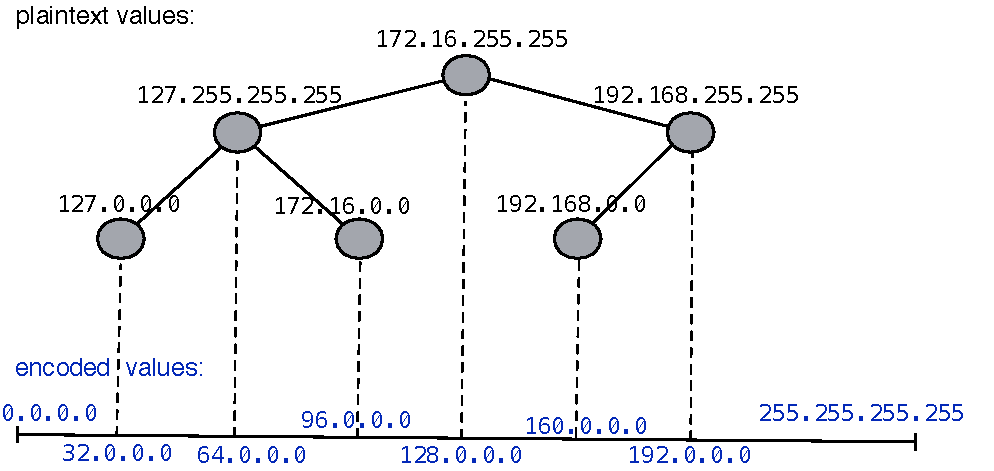
\includegraphics[width=3.45in]{fig/tree}
  \caption{\label{fig:tree} Range match tree. The values of nodes in the tree are the unencrypted IP addresses, and the blue values on the horizontal axis are their encodings. }
\end{figure}



\qu{what happens to collisions w.r.t. port numbers?}
\todo{need to introduce the key k somewhere}

We now explain concretely the API and the implementation of the scheme. 

\subsubsection{Gateway API}

The gateway can use the following functions. 

EncodeRanges encodes the initial ranges. Note that some ranges could consist of
one point only, namely $s = e$. 

% TO CUT TO REDUCE: put all these algorithms into one box

\begin{framed}
\begin{algorithmic}[1]

\Procedure{EncodeRanges}{[$s_1$, $e_1$], $\dots$, [$s_n$, $e_n$]}
  \State Build scapegoat tree on the values 
              $\{s_1, \dots, s_n\}$ 
              $\cup$ $\{e_1, \dots, e_n\}$ 
              $\cup$ $\{-\infty, \infty\}$.
  \State Assign an encoding $\enc(x)$ to each node $x$ in the tree:
  \begin{itemize}
  \item the root gets the middle of the IP range, $e$, 
  \item the left node to the root gets the middle of the range left of $e$ ($e/2$),
  \item the right node gets the middle of the range
  to the right of $e$ ($3e/2$), and so on.
  \end{itemize}

  \State \Return{[$\enc(s_1)$, $\enc(e_1)$], $\dots$, [$\enc(s_n)$, $\enc(e_n)$]}
\EndProcedure

\end{algorithmic}
\end{framed}

EncodeValue encodes the values to be matched against ranges.

\begin{framed}
\begin{algorithmic}[1]

\Procedure{EncodeValue}{$v$}
  \State Search the tree for $v$ to identify the tightest enclosing interval [$p_1$, $p_2$]. 
  \State Let $\low$ and $\high$ be the encodings of $p_1$ and $p_2$. 
  \State Compute $\enc(v) = \low + \prf_k(v)\ \mod\ (\high - \low)$
   \State \Return{$\enc(v)$}
\EndProcedure

\end{algorithmic}
\end{framed}

Note that the search for $p_1$ and $p_2$ is fast, logarithmic time, due to the fact that the 
scapegoat tree is a balanced search tree. 

We now present AddRange and DeleteRange which update the state at the firewall with new rules. 

\begin{framed}
\begin{algorithmic}[1]

\Procedure{AddRange}{$[s, e]$}
  \State Insert $s$ and $e$ in the scapegoat tree. If $s=e$, insert the value only once.
  %	
  \State Initialize $L$ to be the empty list.
  \If{tree needs to be rebalanced}
  	\State Record which nodes change position in the tree during rebalancing, together with 
	their old and new encodings. Namely, record	\[L = \{ \en_1 \leftarrow \en^*_1, \dots, \en_m \rightarrow \en^*_m\},\] where $m$ is the number of nodes who changed position in the tree, and $\en_i$ and $\en^*_i$ are the old and new encoding of the $i$-th node that changed position. 
  \EndIf
  \State Compute  $\enc(s)$ and $\enc(e)$, the encodings of $s$ and $e$, as in EncodeRanges.
   \State \Return{$[\enc(s), \enc(e)], L$}
\EndProcedure

\end{algorithmic}
\end{framed}


Since we are using a scapegoat tree, the number of nodes that change position during rebalancing is amortized worst case $O(\log n)$ where $n$ is the total number of nodes in the scapegoat tree. 

DeleteRange is similar, except that the only result is the list $L$ of changes. 

\subsubsection{Cloud API}

The cloud can run ``$\ge$'' and "$\le$" between any encoded value $\enc(v)$ and encoded enpoint $\enc(s)$ and $\enc(e)$, and obtain a correct answer. Computing $\enc(v_1) < \enc(v_2)$ is meaningless, and returns a random value.


 
\todo{somewhere explain its security with an example -- significantly more secure than enc schemes used in CryptDB, etc}


 






% make differences from mope more clear 

\todo{must emphasize provable guarantees and point to a tech report or something with proofs}
\todo{I think you need to express the security of the scheme again somewhere}


\todo{consistency of encoding vs encryption}




% PROTOCOL

% the gateway encrypts teh IP has to be clear

% Here somewhere we need to discuss that there is one encryption scheme adn then there is how we use it for ports and other ip addresses.

% in the firewall protocol describe how hardware does not change 

% can use the same processing 


%!TEX root = mb.tex
\section{Applications}

\todo{tie all apps in with the two basic operations}

In this section we present how to apply the building blocks to real-world applications.

\section{Application: Firewall}\label{sec:firewall}
We use the term ``firewall'' for stateful and stateless packet filters that filter the traffic based on network layers and transport layers. Stateless firewalls commonly examine the combination of the packet's source and destination address, its protocol, and for TCP/UDP traffic, its source and destination port number. Stateful firewalls additionally keep track of protocol states for each flow and retain packets until they has enough information to make decision. 

In sum, the \RM scheme supports both types of firewalls. The gateway encrypts the rules from the cloud beforehand, and send them back to the cloud. The cloud installs those rules to the firewall. After the initialization is finished, the gateway can encrypt the traffic and forward to the cloud, and the firewall in the cloud can process the traffic normally without modification. When the traffic gets back to the gateway, it gets decrypted.

\subsection{Firewall rules}
Firewalls from different vendors may vary significantly in terms of rule syntaxes and organizations. However,
in general both hardware and software firewalls have a few interfaces. Both ingress and egress of an interface 
can be associated with an access control list (ACL). Each ACL has a number of rules, possibly in the form 
<action, protocol, src ip, src port, dst ip, dst port>. Without loss of generality, we take \texttt{pf}, the 
default firewall under BSD, as an example to illustrate how \sys works with firewalls. Figure \ref{fig:fwrule1} 
shows an example of \texttt{pf} rules. 

\begin{figure}[h]\label{fig:fwrule1}
\begin{lstlisting}[frame=single]
ext_if = "kue0"

block out log quick on $ext_if \
from 157.161.48.0/24 to any

block in quick on $ext_if \
from any to 255.255.255.255

pass out on $ext_if proto tcp \
from any to any port 80
\end{lstlisting}
\caption{\texttt{pf} configuration example}
\end{figure}

To work with \sys, we need to rewrite the rules above. Using the \RM scheme, we encrypt all IP addresses, prefixes, and port numbers inside the rules. Note that \texttt{any} is the alias of \texttt{0.0.0.0/0}. Recall that in Section \ref{sec:range} we want to keep the chance of collision as low as possible, therefore we map the IPv4 addresses into the IPv6 space before encoding those values. For example, to encrypt the IP prefix \texttt{157.161.48.0/24}, the gateway first extends it to \texttt{::ffff:157.161.48.0/120}.
Now the prefix represents the range from \texttt{::ffff:157.161.48.0} to \texttt{::ffff:157.161.48.255}. The gateway then insert
both endpoints to the tree, and gets their encrypted values. 

Suppose those two values are \texttt{fd6a:1faf:577b:bee4:0:0:0:0} and
\texttt{fd6a:1faf:577b:bee4:0:1:0:1}. Note that we can't represent this range using a single prefix, instead it has to be 
represented by at least two prefixes (\texttt{fd6a:1faf:577b:bee4:0:0:0:0/96} and \texttt{fd6a:1faf:577b:bee4:0:1:0:0/127}).
In this case, we have to split the original rule into 2 new rules:

\begin{lstlisting}[frame=single]
block out log quick on $ext_if \
from fd6a:1faf:577b:bee4:0:0:0:0/96 to any

block out log quick on $ext_if \
from fd6a:1faf:577b:bee4:0:1:0:0/127 to any
\end{lstlisting}

\todo{evaluate how many additional new rules are needed.}

After the gateway has rewritten the rules, it sends the rules back to the firewall on the cloud so that the
firewall can filter packets using the new rules.

\subsection{Encryption and decryption}
Every time the gateway forwards a packet from the user, it replace the IPv4 header with the IPv6 header 
using the Stateless IP/ICMP Translation (SIIT) algorithm \cite{rfc2765}. The purpose of this operation is to leave 
enough address space for avoiding address collision. The gateway then encrypts the source IP, source port, 
destination IP, destination port fields using the Range Match scheme in Section \ref{sec:range}.

\todo{a diagram that shows the packet format before and after encryption}

\subsection{Remark}
A key feature of our scheme is that we don't require to change the firewall implementations. As we discussed in Section \ref{sec:range}, the central 
piece of firewalls is packet classification, which is essentially a problem of finding a hyper-rectangle that contains a point from a given set of hyper-rectangles. Our \RM scheme keeps the order among the coordinates of hyper-rectangles, and the order between the coordinates of hyper-rectangles and points. In other words, their topological relations are preserved. Therefore existing firewalls can still work with \sys without modification. This property is important, since many high-speed firewalls are implemented in hardware, which is difficult and expensive to redesign.

\section{Application: NAT}\label{sec:nat}

give example of what a rule becomes

\section{Application: IDS}\label{sec:ids}
Unlike the previously presented middleboxes, devices which perform Intrusion Detection/Prevention (IDS/IPS) operate over the TCP bytestream, not just over packets and headers independently.
For IDSes, reconstructing the TCP bytestream allows the middlebox to detect attack strings which may span two or more packets.
Many other `stateful DPI' devices reconstruct the TCP bytestream while allowing packets to pass through, such as application firewalls and parental filters.
Due to this reconstruction cost, devices which perform stateful DPI typically provide much lower throughput than devices which perform
solely on headers -- for example~\todo{cite some industrial boxes here}.
Other devices also operate at the bytestream abstraction by terminating the TCP connection, \eg{} HTTP proxies, which must cache entire images (which would normally be divided across multiple packets). 

As we have seen with the previous middleboxes (Firewalls, NAT, Load Balancers), the \sys gateway can support middleboxes which operate on a packet-by-packet basis while similarly remaining stateless and operating on a packet-by-packet basis itself.
To support IDSes, however, we must use a modified gateway which supports bytestream-aware middleboxes by reconstructing the TCP flow at the middlebox.
As we show in~\S\ref{sec:eval}, the stateful gateway achieves lower throughput than the stateless one.
Fortunately, not all bytestream-aware middleboxes require a stateful, bytestream-aware gateway. 
As we shall see, some HTTP proxies -- proxies for non-pipelined HTTP requests -- can be fully supported with a stateless \sys gateway (pipelined HTTP proxies, however, do require a stateful gateway).

\sys's IDS is based on BlindBox~\cite{blindbox}, an IDS which 

\section{Application: Proxy/cache}\label{s:proxy}
\todo{Cut out any of this, it's leftover text from something I tried that didn't work but didn't want to delete in cas it winds up being helpful}
They also {\it terminate} connections rather than allowing packets to ``pass through''.
When a client opens a new HTTP connection, a typical proxy will capture the client's SYN packet and open a new connection to the client, as if it were the web server the client wished to connect to. 
The proxy then opens a second connection in the background to the original web server, as if it were the client. 
Multiple clients may attempt to access the same web page through the proxy, in which case, the proxy maintains multiple client-facing connections, but one or few persistent server-facing connections.
When a client sends a request for new content, the proxy can either forward the request to the web server, or, the proxy may serve the content from its {\it cache} -- images and content that other clients have already requested which the proxy then stored locally. 
Caching improves client-perceived performance because content is served from the proxy, which is closer to the client than the web server.

In order to understand what content the client is requesting (index.html from google.com, photo.jpg from flickr.com, \etc{}), the proxy must parse the HTTP header, which, unlike IP/TCP/UDP headers is variable-length (\eg{}, URLs may be any number of characters long, while port numbers are always 16 bytes long) and variable-offset (\eg{}, the IP source always appears 12 bytes from the beginning of the packet, where the HTTP method may appear anywhere within an HTTP payload).

\sys implements web proxying using the keyword match encryption algorithm. 
However, rather than encrypting fixed values at fixed locations, the \sys gateway parses the HTTP header to determine what data to encrypt.
Nevertheless, as we show in \S\ref{sec:eval}, this parsing has a negligible overhead on gateway throughput -- less than 1\% when added in addition to the existing encryption required for Firewalling and NAT.
We implement two versions of gateway encryption: one which uses the stateless gateway and can encode HTTP requests which are not pipelined, and one which uses the stateful gateway, which supports pipelined HTTP requests as well (we discuss the difference as follows).

First case: unpipelined. HTTP header is **always** the first few bytes in the first packet sent by the client -- so easy to know where to start parsing.
\begin{itemize}
\item architecture overview
\item HTTP request -- absolute url and Host + relative url
\item tokenization special case \\
    \begin{itemize}
    \item in order to fetch the url from the header
    \item tokenize HTTP methods: GET, POST, ...
    \item tokenize attribute names: "Host:"
    \item tokenize versions: "HTTP/1.1", ...
    \end{itemize}
\item walk through the whole process
\item do not support pipelining yet
\end{itemize}

- may want to say that it has an index for seaching fast the url which it can thanks to the det scheme


we are focusing on the transparent proxy
- discuss the kind of proxies we are focusing on

proxies have two benefits: latency savings which aplomb gives you 
and bandwidth savings, which aplomb does nogive you
 
L7 Proxy / Cache

explain how the proxy finds if there is  a match --looks at header bytes
extra field attached to the packet -- gateway understands http and points out file id, 

discuss both cases: cache miss and hit

- two indep tcp connections 

how to populate the cache: content providers pushing the content to CDNs, or the gateway understands
http and tags what is content and what is ID
oops justine forgot to mention this above

the web proxy needs to send http response 

proxy only looks at the top N bits corresponding to a large header and matches the file id with the entire path
and matches GET and a few others -- avoid parsing http this way


discuss how the proxy can reconstruct the response?
can proxy reconstruct the ip header and the http header  and the tcp header without being able to encrypt
--- check the http header details

With pipelined requests, we don't have the header is always the first part of the packet. Instead, we need to {\it reconstruct the payload} to tell where to parse. This is where we need to use the other gatway. Otherwise, the functionality is exactly the same above -- only now we operate on the reconstructed payload rather than the first few bytes of the first packet.


\section{Application: Intrusion Detection}
Like proxies, Intrusion Detection/Prevention systems operate over packet payloads, not just the IP/TCP/UDP headers.
IDS/IPS are canonical examples of DPI devices.


\section{Other middleboxes}\label{sec:vpn} \label{sec:other_apps} \label{sec:not_supp}\label{sec:loadb}
\qu{should we call them applications or middleboxes in the sections above?}


L4 load balancer
L7 load balancer

-- VPN naturally remains the same. 

-- make the tables of applications consistent with each other and make sure we support all 

-- what is difference between L4 and L7 load balancer -- do we need both?

-- IP forwarding app, what is that?

-- how about the application firewall?

-- discuss wan optimizers and compression, that aplomb does not really support them in the basic model (requiring this special model that is not quite aplomb) -- also the conflicts it would show up for us


\section{Putting all together}\label{sec:all}

Putting them together
new packet structure

%!TEX root = mb.tex

\section{System implementation} \label{sec:impl}
\eat{
\todo{this is important to write properly because it is a systems paper and there were some nontrivial decisions}.

Things to cover:

- gateway and middlebox implementation

- explain why the firewall hardware does not change (or was that above?)

- second flow udp/tcp

- might want to explain these points made in intro: "
Sylvia, it would be great if you could read and revise the paper. Feel free to edit directly in tex!
We really need your feedback at this stage."

- new packet structure and headers -- multiple layers of headers? graph? (there is some text and a figure in a google doc about this)

- some things are specific to web proxy from what I remember
}

We now describe the \sys architecture and implementation. 
As discussed in \S\ref{sec:overview}, \sys redirects traffic to the cloud and back for {\it middlebox processing} using a {\it redirection gateway}.
%\todo{Put a little overview aout gateway, metadata channel, mbs here???}
We now present the implementation and architecture of the redirection gateway (\S\ref{sec:gateway}), followed by the modifications we made to middleboxes to support \sys (\S\ref{sec:middleboxes}).
%Finally, we discuss our EC2 deployment of these components (\S\ref{sec:deployment}).


\subsection{Redirection \& gateway implementation}
\label{sec:gateway}

\begin{figure}[t]
  \centering
  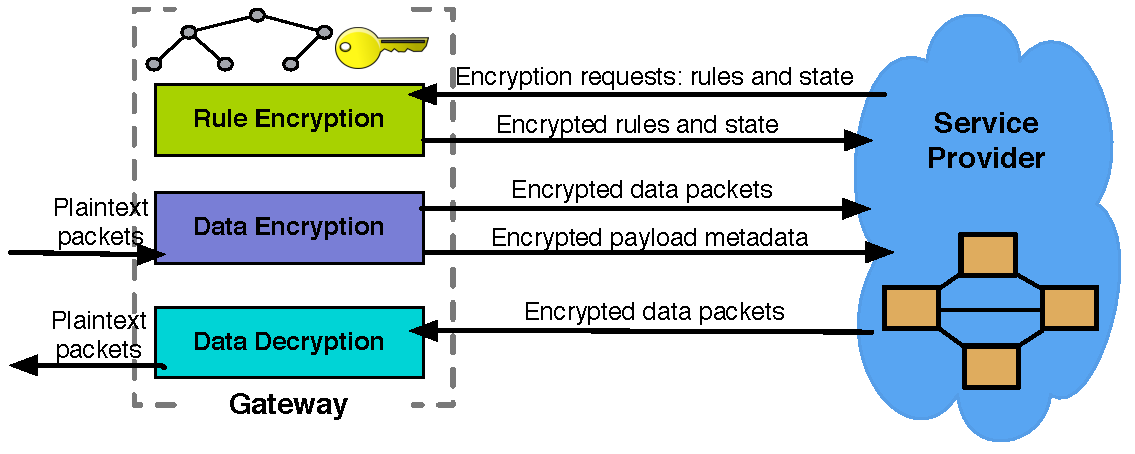
\includegraphics[width=3.25in]{fig/gateway2cloud}
  \caption[]{\label{fig:gatewaymeta} Communication between the cloud and gateway services: rule encryption, data encryption, and data decryption}
\end{figure}



\begin{figure}[t]
  \centering
  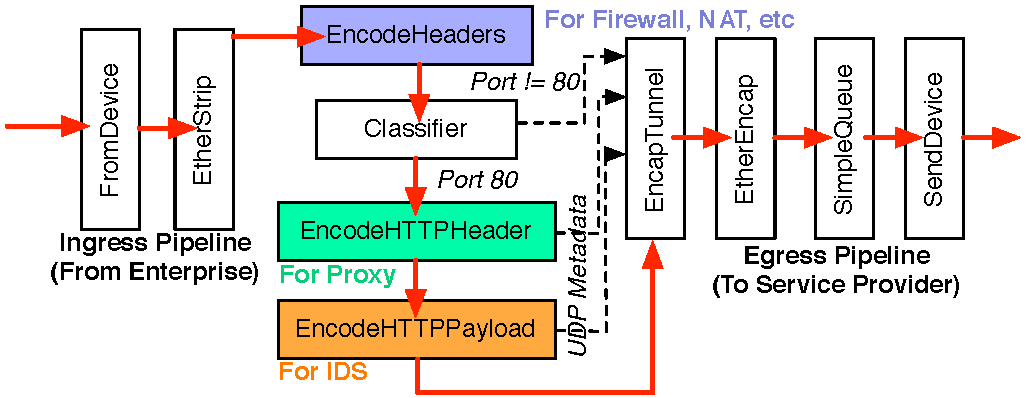
\includegraphics[width=3.25in]{fig/gatewaydiag}
  \caption[]{\label{fig:gateway} Data encryption (enterprise to cloud) click module.}
\end{figure}

The gateway serves two purposes. First, it redirects traffic to/from the cloud for middlebox processing. Second, it provides the cloud with encryptions of IDS/FW rulesets and updates to the RangeMatch tree.
Every gateway is configured statically to tunnel traffic to a fixed IP address at a single service provider point of presence.
A gateway can be logically thought of as three services: the rule encryption service, the pipeline from the enterprise to the cloud (Data encryption), and the pipeline from the cloud to the enterprise (Data decryption). 
All three services share access to the RangeMatch tree and the private key $k$.
Figure~\ref{fig:gatewaymeta} illustrates  these three services and the data they send to and from the cloud provider.

\noindent{\bf Rule Encryption.} The rule encryption component provides the cloud provider with encrypted rules/policies to use at the middlebox. 
There are two possible ways rules can be generated. First, an enterprise may choose to generate their own rules, in which case, they send encrypted versions of the rules directly to the cloud.
Rules can contain IP addresses, port numbers, and substrings of attack signatures; the first two must be encrypted with both keyword match and range match, the last needs only to be encrypted with keyword match.
Alternately, the enterprise may opt in to a `default' set of rules from the cloud provider, in which case the cloud provider sends the rules to the gateway which encrypts them and sends them back.
The rule encryption component also sends rule updates. Whenever an adjustment is made to the RangeMatch table, it sends an update to the cloud provider with the adjusted mappings/rules.
If the gateway ever changes its key, the encryption component must also signal to the cloud provider and re-encrypt all rules.
%\todo{too high level? Details about how updates work?}

\noindent{\bf Data Encryption.} In Figure~\ref{fig:gateway}, we show the DPDK-Click~\cite{click} packet processing pipeline that implements data encryption and transmits packets from the enterprise to the cloud.
Traffic that is returning from the Internet and traffic that is about to be sent to the Internet are both sent along this pipeline.
This figure assumes the enterprise is already using IPv6, if it is not, the pipeline would also include a `4to6' element.
In \S\ref{sec:overview}, we described how \sys encodes packet content using the AES, Keyword Match, and Range Match encryption algorithms. 
The encrypted values are placed either directly back in to a data packet, or transmitted over a {\it metadata channel}.

Below, we detail the three elements we implemented to encrypt the packet data:

\noindent {\it Encode Headers:} Encrypts the IP, TCP, and UDP headers, replacing all IP and Port numbers in the packet with values calculated using the {\it RangeMatch} encryption algorithm. Appends the AES-encrypted values to the IP options field of the data packet.
Required to support all middleboxes. 

\noindent {\it Encode HTTP Header.} Encrypts the HTTP header for {\it the first GET request only.} Does not modify the data packet itself, but instead places the keyword match encryptions of the values in a new packet sent over the metadata channel. \clan{Here! And we also mention this in Section 8.2}
The new packet marks (a) the encrypted 5-tuple flow ID for the packet, (b) that this is HTTP GET data for the proxy, and (c) the encrypted values. At the cloud, the proxy can read this metadata channel to obtain the encrypted URL for the GET request and check its cache for the encrypted data. This element is only needed if there is an HTTP proxy enabled at the cloud, otherwise it can be disabled at the gateway.

\noindent {\it Encode HTTP Payload.} Encrypts the entire HTTP payload (as described in \S\ref{sec:ids}), placing the keyword match values in a new packet in the metadata channel. Unlike the other two elements, this element keeps per-flow state, reconstructing the TCP stream in order to generate keyword match tokens for keywords which are divided across two subsequent packets.  The metadata channel packets contain (a) the encrypted 5-tuple for the packet, (b) that the packet contains keyword match data for the IDS, and (c) the encrypted values. At the cloud, the IDS can read this metadata channel to detect attacks; if there is a match it instructs the firewall to block the 5-tuple for the flow. This element is only needed if there is an IDS enabled at the cloud, otherwise it can be disabled at the gateway.


\noindent{\bf Data Decryption.} Packets returning from the cloud follow a much simpler packet processing pipeline than those being encrypted.
The packet payloads are decrypted using standard AES; the IP and port values from the options header are decrypted and then copied in to the packet header. The options header is removed.
If the enterprise is running IPv4, the traffic is sent back through the 4to6 converter to convert the packet back to IPv4.
The packet is then sent out to the Internet or the client at the enterprise.


\subsection{Middlebox implementations}
\label{sec:middleboxes}

\begin{figure}[t]
  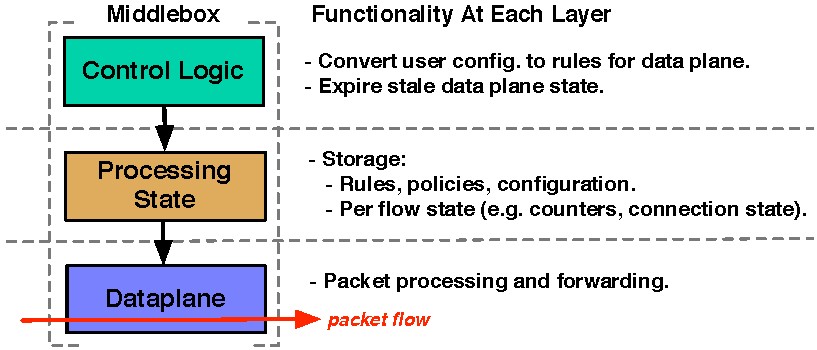
\includegraphics[width=3.25in]{fig/mbarch}
  \caption[]{\label{fig:mbarch} Typical middlebox software components. For most middleboxes, packet processing operations in the dataplane remain unmodified by \sys.}
\end{figure}

We implemented \sys for all middleboxes listed in Table~\ref{tab:apps-ops} using DPDK-Click~\cite{click}, with varying levels of modification to a baseline (unencrypted) design required to make them compatible with \sys. 
Figure~\ref{fig:mbarch} guides our discussion of these changes. %Most middlebox codebases can be divided in to three categories of functionality.
Although  middlebox software architectures are unlikely to be cleanly divided in to three independent components as shown, most classes and functions within a middlebox codebase can be labeled as one of these three categories.
These categories are: the dataplane (which performs packet processing), the middlebox state (which stores and updates rules and policies, as well as per-flow state like counters and connection state), and the control logic (which converts user configurations to rules and policies, and updates/refreshes state). 
Importantly, packet processing only occurs in dataplane functions, which are usually tightly engineered to process each packet in microseconds or faster.

We adapted all header-only middleboxes {\it without modifying steady-state dataplane functions}, and hence preserving the performance properties of the existing middleboxes.
We were able to do this because the encrypted values in the IPv6 header are stored in the normal IPv6 header formats, and because our encryption schemes preserve the exact match and range match semantics these devices use to operate correctly.
All we need to do to be compatible with normal dataplane behavior is to encrypt all values in the rules and configuration files using the the range match encryption algorithm.

We do need to change the control logic and add one `special case' check to the dataplane; this is to handle rule {\it updates}. 
The update code is triggered rarely -- when the gateway changes its key $k$, or when there is an update to the Range Match tree.
In this case the rules must be re-encrypted, and any per-session state (\eg{} the flow table in the NAT) must be re-encrypted as well.
When such an update is about to occur, the gateway first re-computes all rules {\it before} it begins to use the new encryption values on traffic. It signals to the cloud provider that it is about to perform a rule update. Then, all middleboxes transmit their rules / state tables to the gateway for re-encryption. 
Once all middleboxes have received their updated rules and state, the gateway `switches' to the new ruleset, sending a signal packet in the dataplane. When a middlebox receives this signal packet (the only change we make to the dataplane is to check for this signal packet) it switches out the ruleset to use the new values.~\footnote{\small There is a race condition for the flow state: consider a SYN packet which arrives just before the signal packet at a NAT. The NAT will encode the SYN packet in its state table using the old encryption scheme, and then immediately need to switch over to the new encryption scheme -- before it has the new mapping for the new flow. The middlebox will then immediately request a new encryption for the rule. Hence, a small number of packets may be misclassified during the transition.}
\todo{This is ugly as sin! Sigh! Can we do better?}  

Bytestream-aware middleboxes require changes in the dataplane as well as the control logic: \sys makes reading the payload directly impossible, and hence these middleboxes must be modified to operate over the metadata channel instead.
We re-implemented all such middleboxes from scratch.
However, these changes need not be a performance penalty: as we show in \S\ref{sec:eval}, we wrote an HTTP proxy from scratch to cache HTTP content; this proxy achieves comparable performance to existing, unencrypted proxies despite our encryption.
The primary difference between our proxy and a standard implementation is that the `table' storing file names/URIs and the file data is now over encrypted values; the content served is also opaque, encrypted data. 
In addition, the file names/URIs are read from the metadata channel, rather than the primary connection with the data packets. 
Otherwise, much of the more complicated aspects of the codebase (\eg{}, TCP session termination, storage and cache optimization, etc) can be implemented using out of the box libraries.



%!TEX root = mb.tex

\section{Evaluation} \label{sec:eval}

As we showed in \S\ref{sec:impl}, \sys supports all middlebox applications in typical outsourcing environments~\cite{aplomb,nfv} -- including header-only middleboxes as well as bytestream-aware middleboxes . 
Hence, from a functionality perspective, \sys answers our original question, ``Is it possible to enable a third party to perform traffic processing for an enterprise, {\em without seeing the enterprise's traffic}?''  strongly in the affirmative.

To evaluate \sys more deeply, we now investigate whether \sys is practical from a performance perspective, looking at the overheads due to encryption (over the header or the payload) and redirection. 
Overall, we find that \sys provides client performance comparable to APLOMB~\cite{aplomb} -- e.g., page load times increase by \todo{foo}\% relative to APLOMB when caching is disabled, and by \todo{bar\%} when caching is enabled.
System efficiency varies dramatically between Header-Only \sys and Bytestream-aware\sys.
Header-only \sys reduces gateway throughput by \todo{foo\%} relative to APLOMB~\cite{aplomb} and has zero overhead at the outsourced middleboxes. 
Bytestream-aware \sys enabled imposes a higher overhead, with the gateway able to forward \todo{bar\%} fewer Gbps than \sys without bytestream reconstruction.

We ran our experiments using the implementation described in \ref{sec:impl}. 
For most experiments, we use a synthetic workload generated by the DPDK PacketGen~\cite{pktgen}; for experiments where an empirical trace is specified we use the m57 patents trace~\cite{patents} and the ICTF 2010 trace~\cite{ictf}.

\subsection{End-to-End Performance}
We first inspect end-to-end client performance when traffic is redirected through \sys.

\begin{figure}
  \hspace{-15pt}
  \begin{tabular}{cccc}
  
\includegraphics[height=1in]{fig/cdflabel}
  &\hspace{-10pt}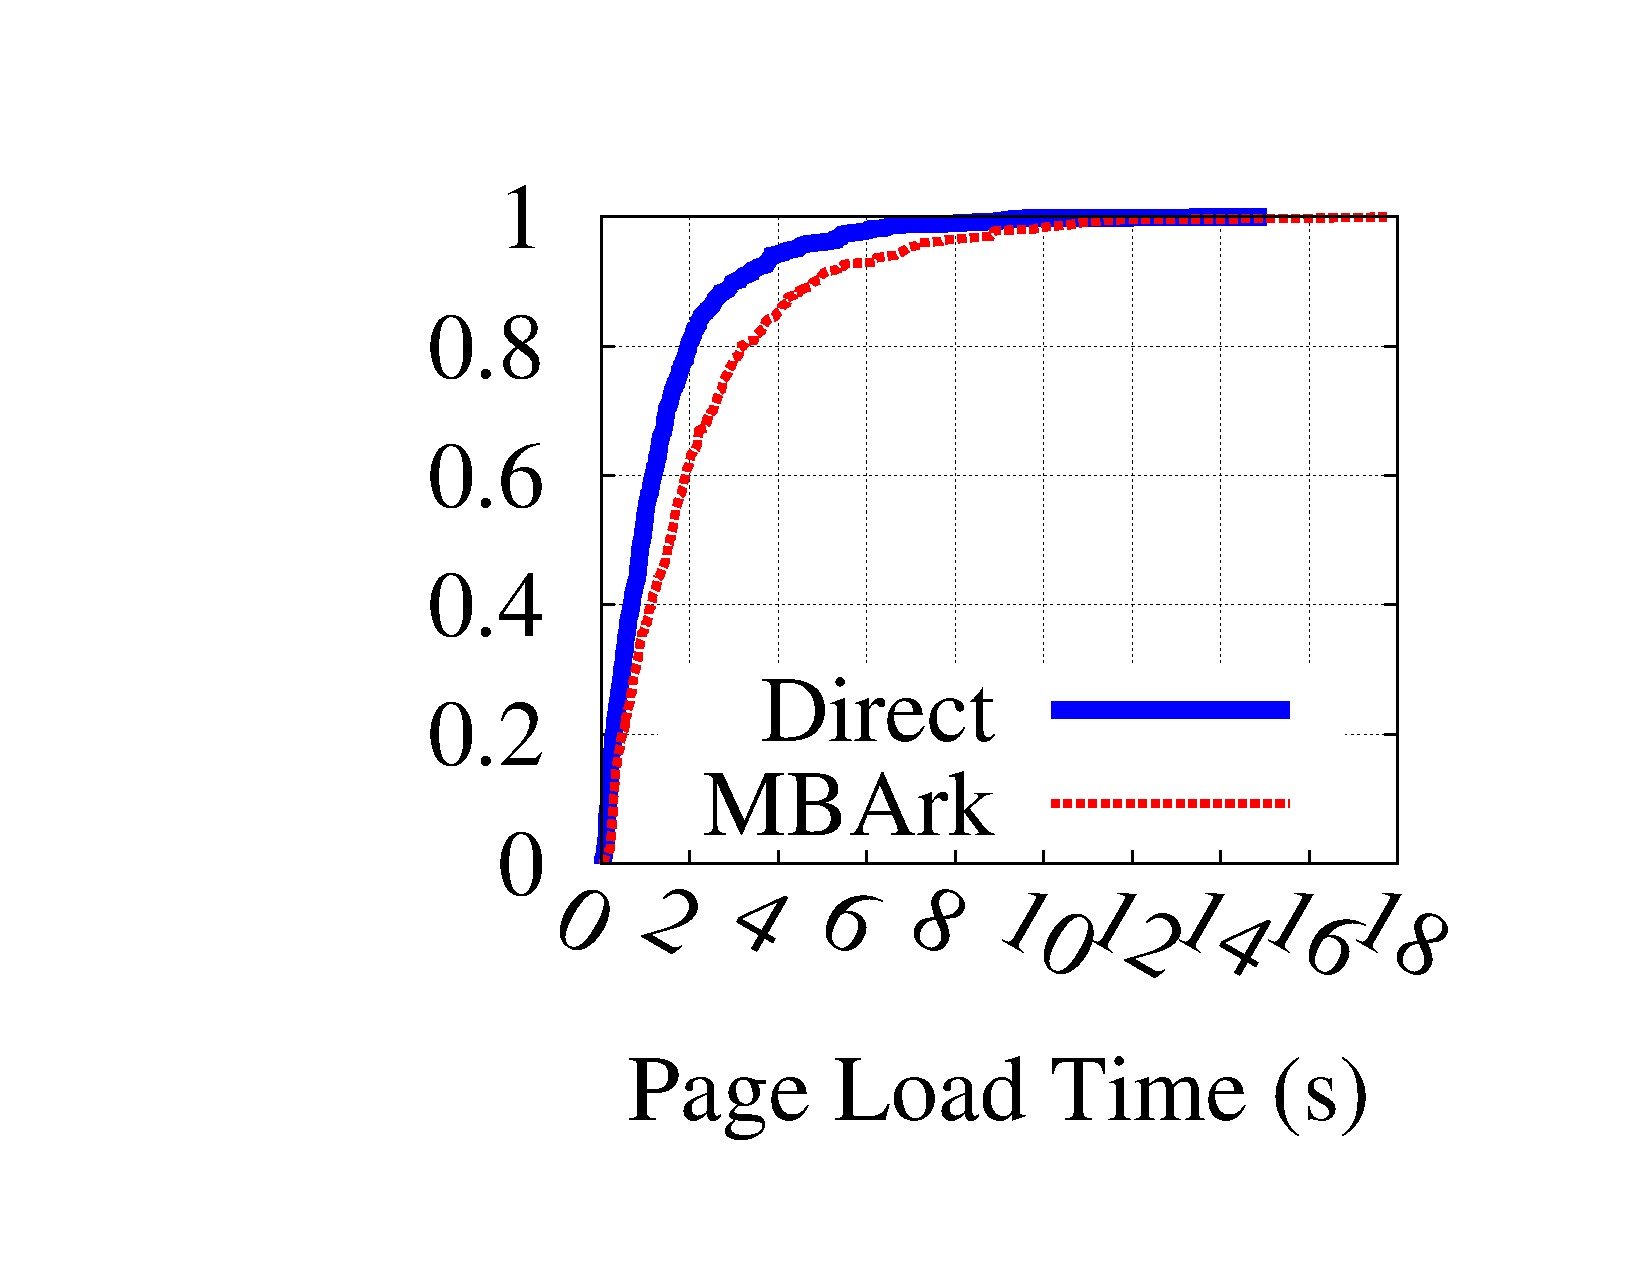
\includegraphics[height=1in]{fig/e2e_loadtimes}
  &\hspace{-10pt}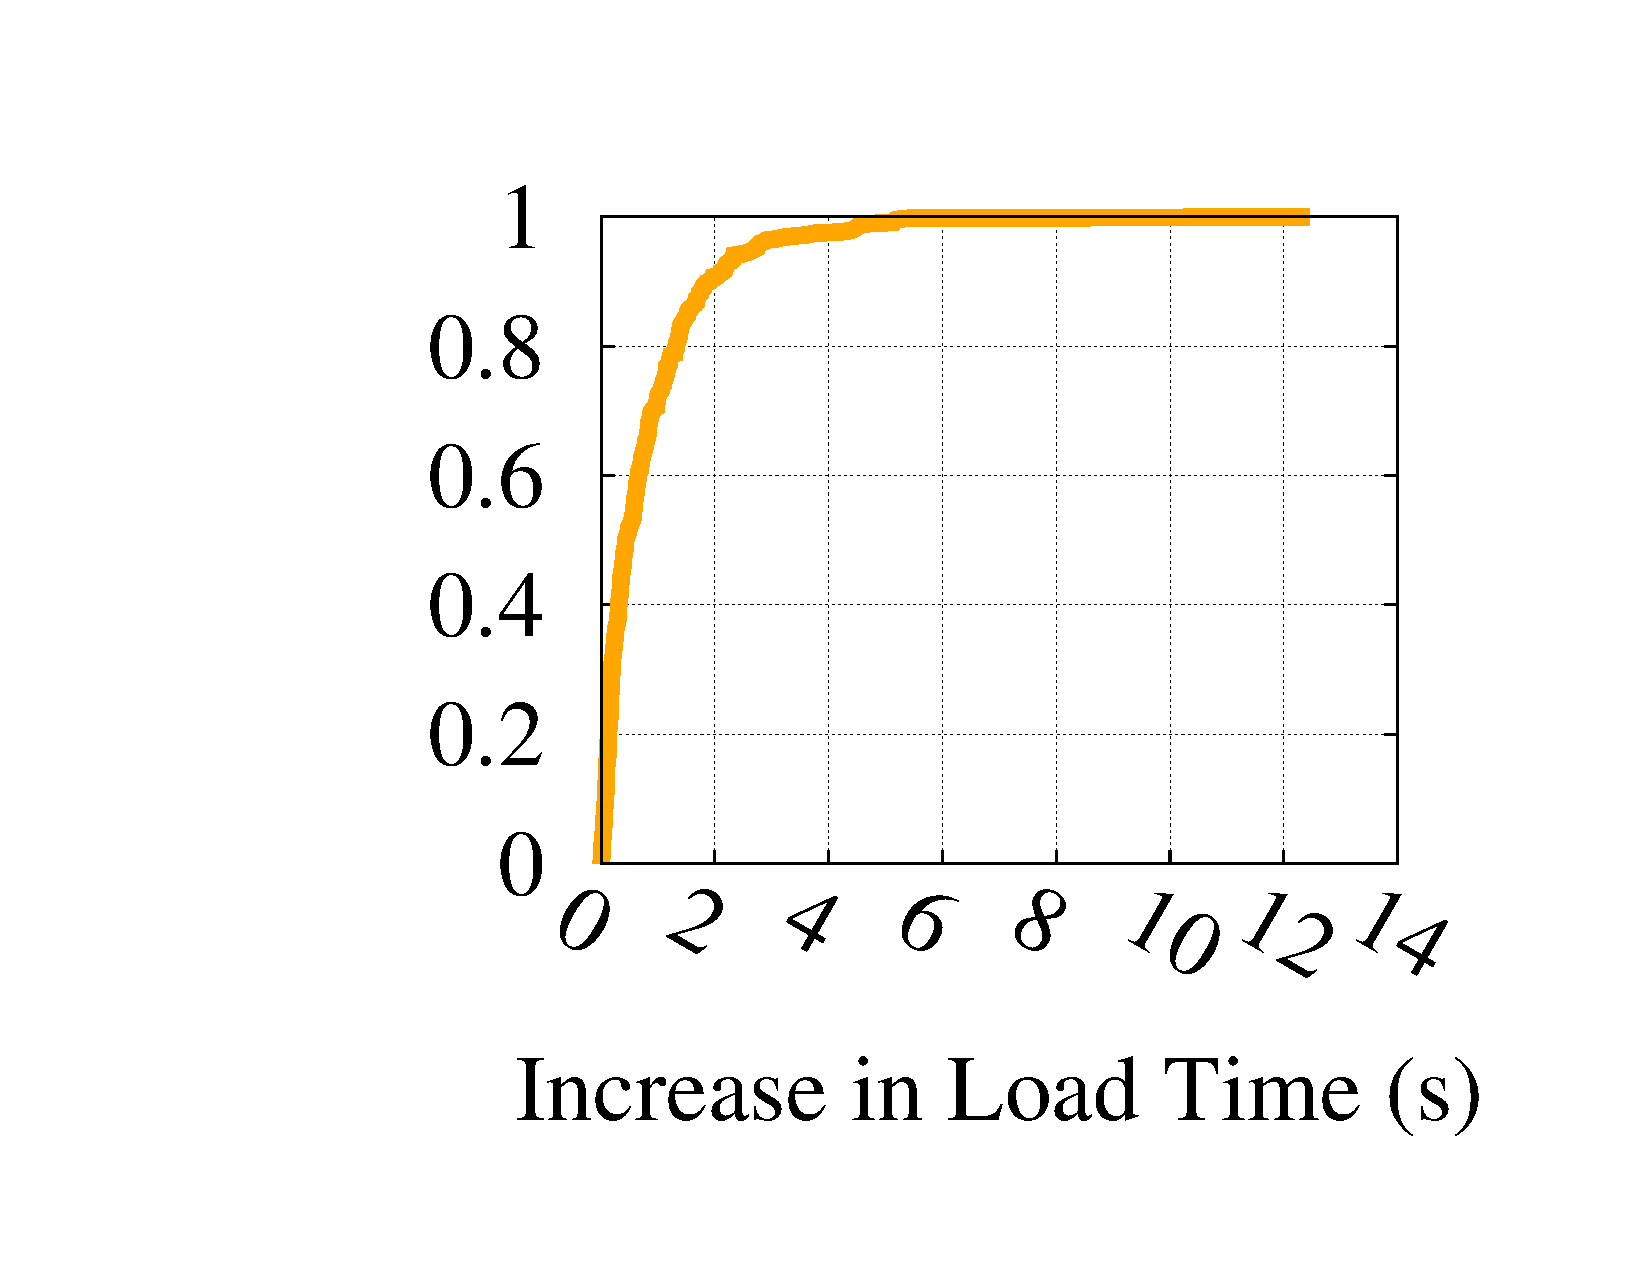
\includegraphics[height=1in]{fig/e2e_delta_absolute}
  &\hspace{-10pt}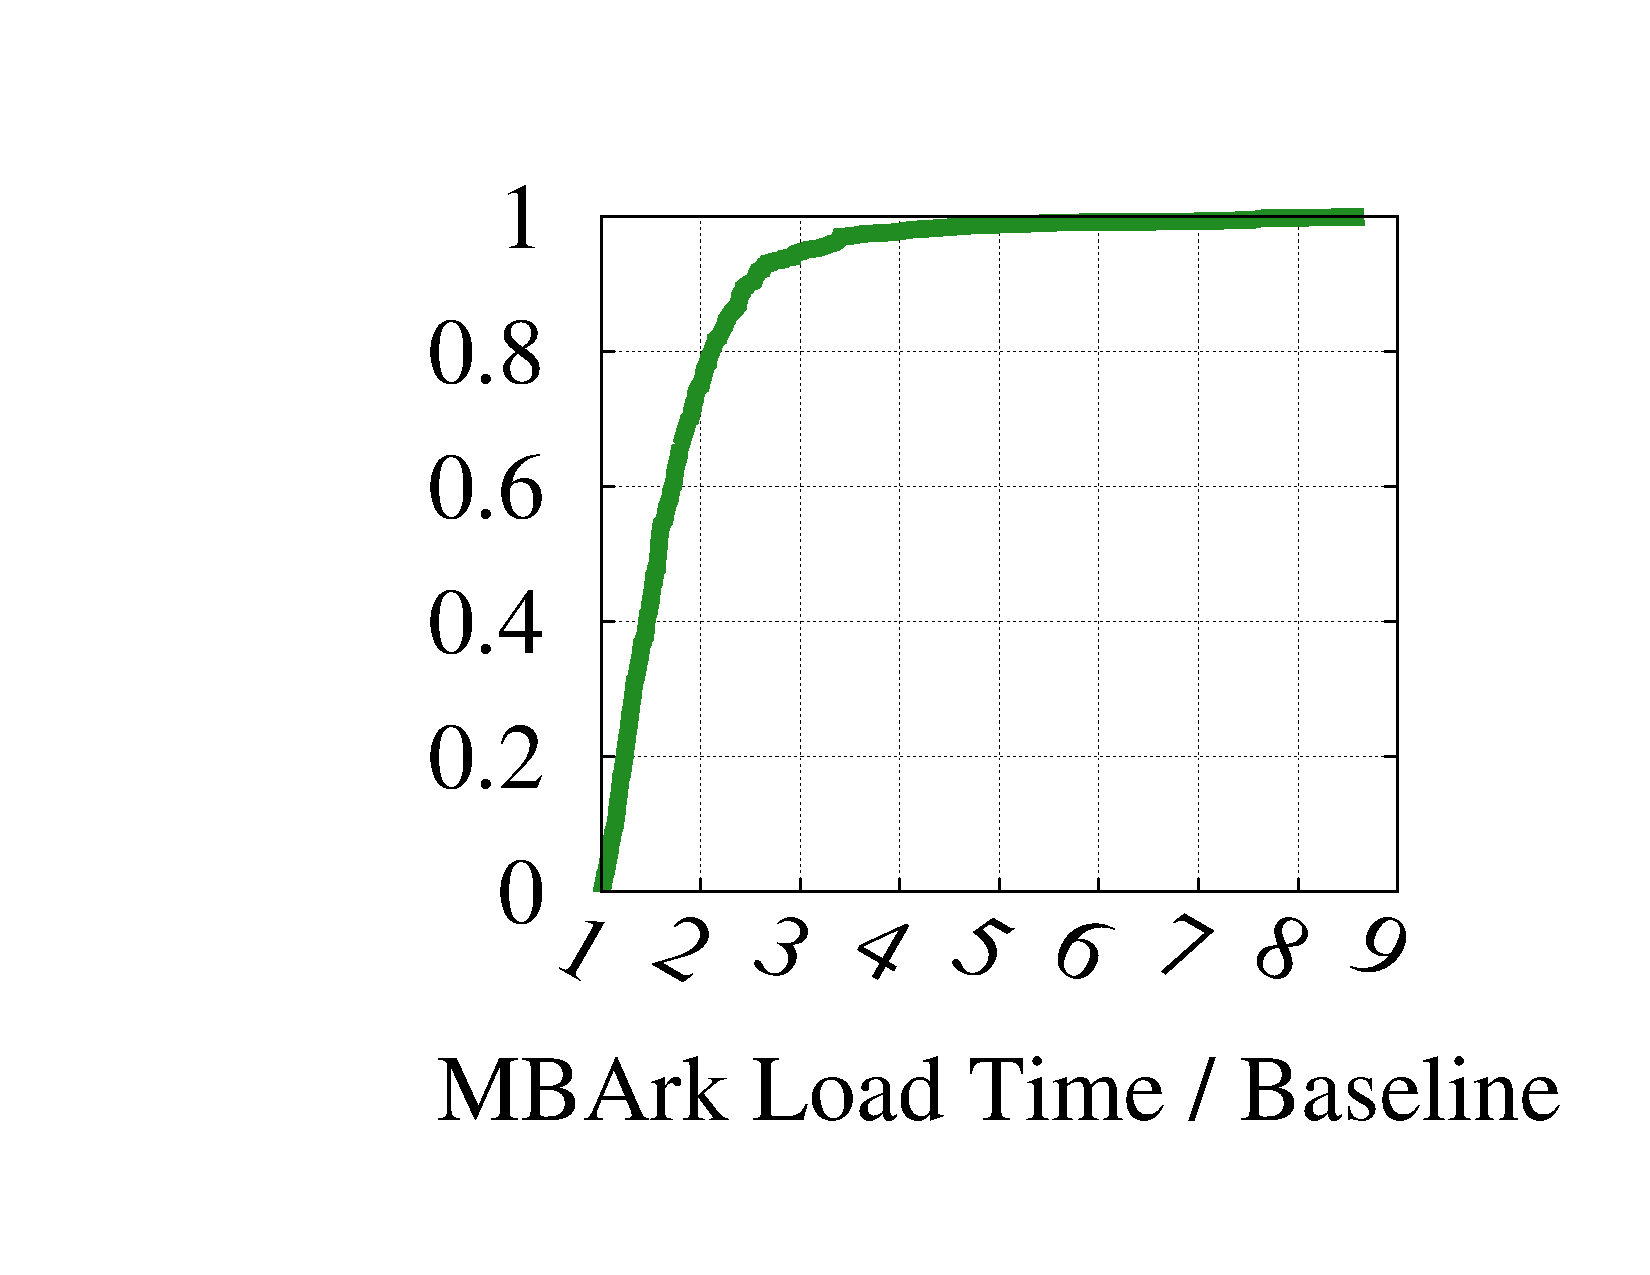
\includegraphics[height=1in]{fig/e2e_delta_relative}
  \\
  &(a)&(b)&(c)\\
  \end{tabular}
  \caption[]{\label{fig:e2eloads} Page load times through \sys compared to direct download.}
\end{figure}
{\it What overheads does \sys impose on web download times?}
\todo{CL}

{\it How much does bandwidth increase between the gateway and the cloud from using \sys? How much would this bandwidth increase an enterprises networking costs?}
\sys sends all network traffic to and from the middlebox service provider for processing, before sending that traffic out to the Internet at large. In NFV contexts, the clients' middlebox service provider and network connectivity provider are one and the same and one might expect costs for relaying the traffic to and from the middleboxes to be rolled in to one `package.' 
However, in the APLOMB setting, the middlebox service provider is a cloud, meaning that the client must pay a third party ISP to transfer the data to and from the cloud, before paying that ISP a third time actually transfer the data over the network.

Beyond sending the primary traffic 3 times (2$\times$ on the uplink, $1\times$ on the downlink), the gateway also inflates the size of this traffic due to encryption overhead:
\begin{itemize}
  \item If the enterprise uses IPv4, there is a 20-byte per-packet cost to convert from IPv4 to IPv6. If the enterprise uses IPv6 by default, there is no such cost.
  \item If HTTP proxying is enabled, there are on average 132 bytes per request in additional encrypted data.
  \item If HTTP IDS is enabled, there is at worst a 5$\times$ overhead on all HTTP payloads.
\end{itemize}
We used the m57 trace to understand how these overheads would play out in aggregate for an enterprise.
On the uplink, from the gateway to the middlebox service provider, traffic would increase by 2.5\% due to encryption costs for a Header-Only Gateway. Traffic would increase by 4.3$\times$ on the uplink for a bytestream-aware gateway. 

Using current bandwidth pricing~\cite{comcast-costs, megapath-costs, verizon-costs}, we can observe how such inflation would increase costs: 
\todo{Getting frustrated with these numbers so leaving them here and will come back to them. Megapath offers a dedicated link at 5x5Mbps for \$250/mo; 20x20Mbps for \$1300/mo. Comcast offers enterprise cable at 150/20Mbps for \$250/mo. The three way bounce should result in a cost increase of 15-50\%, depending on how much the internal link is providioned for. The DPI should be 2-3 times that, so, between 30-150\%... 
}

\subsection{Header-Only \sys}
We first evaluate Header-only \sys, with its stateless gateway. 
Header-only \sys supports all middleboxes which operate only on IP and TCP headers (\eg{}, firewalls, NATs, and L4 Load Balancers) , as well as proxies for non-pipelined HTTP connections (as discussed in \S\ref{sec:proxy}).
The primary cost at the gateway comes from implementing the range encryption algorithm we developed in~\ref{sec:rangematch}. 
Unlike existing order preserving algorithms~\cite{mope,BCLO} which require on the order of milliseconds for every encryption operation, range encryption can keep up with packet processing workloads, requiring only 3$\mu$s per packet to encrypt (three orders of magnitude faster than previous approaches).
We discuss the range match scheme and the gateway in the following subsection, after which we present the performance of individual middleboxes when modified for \sys.

\subsubsection{Header-Only Gateway}
\begin{figure}[t]
  \centering
  \begin{tabular}{cc}
  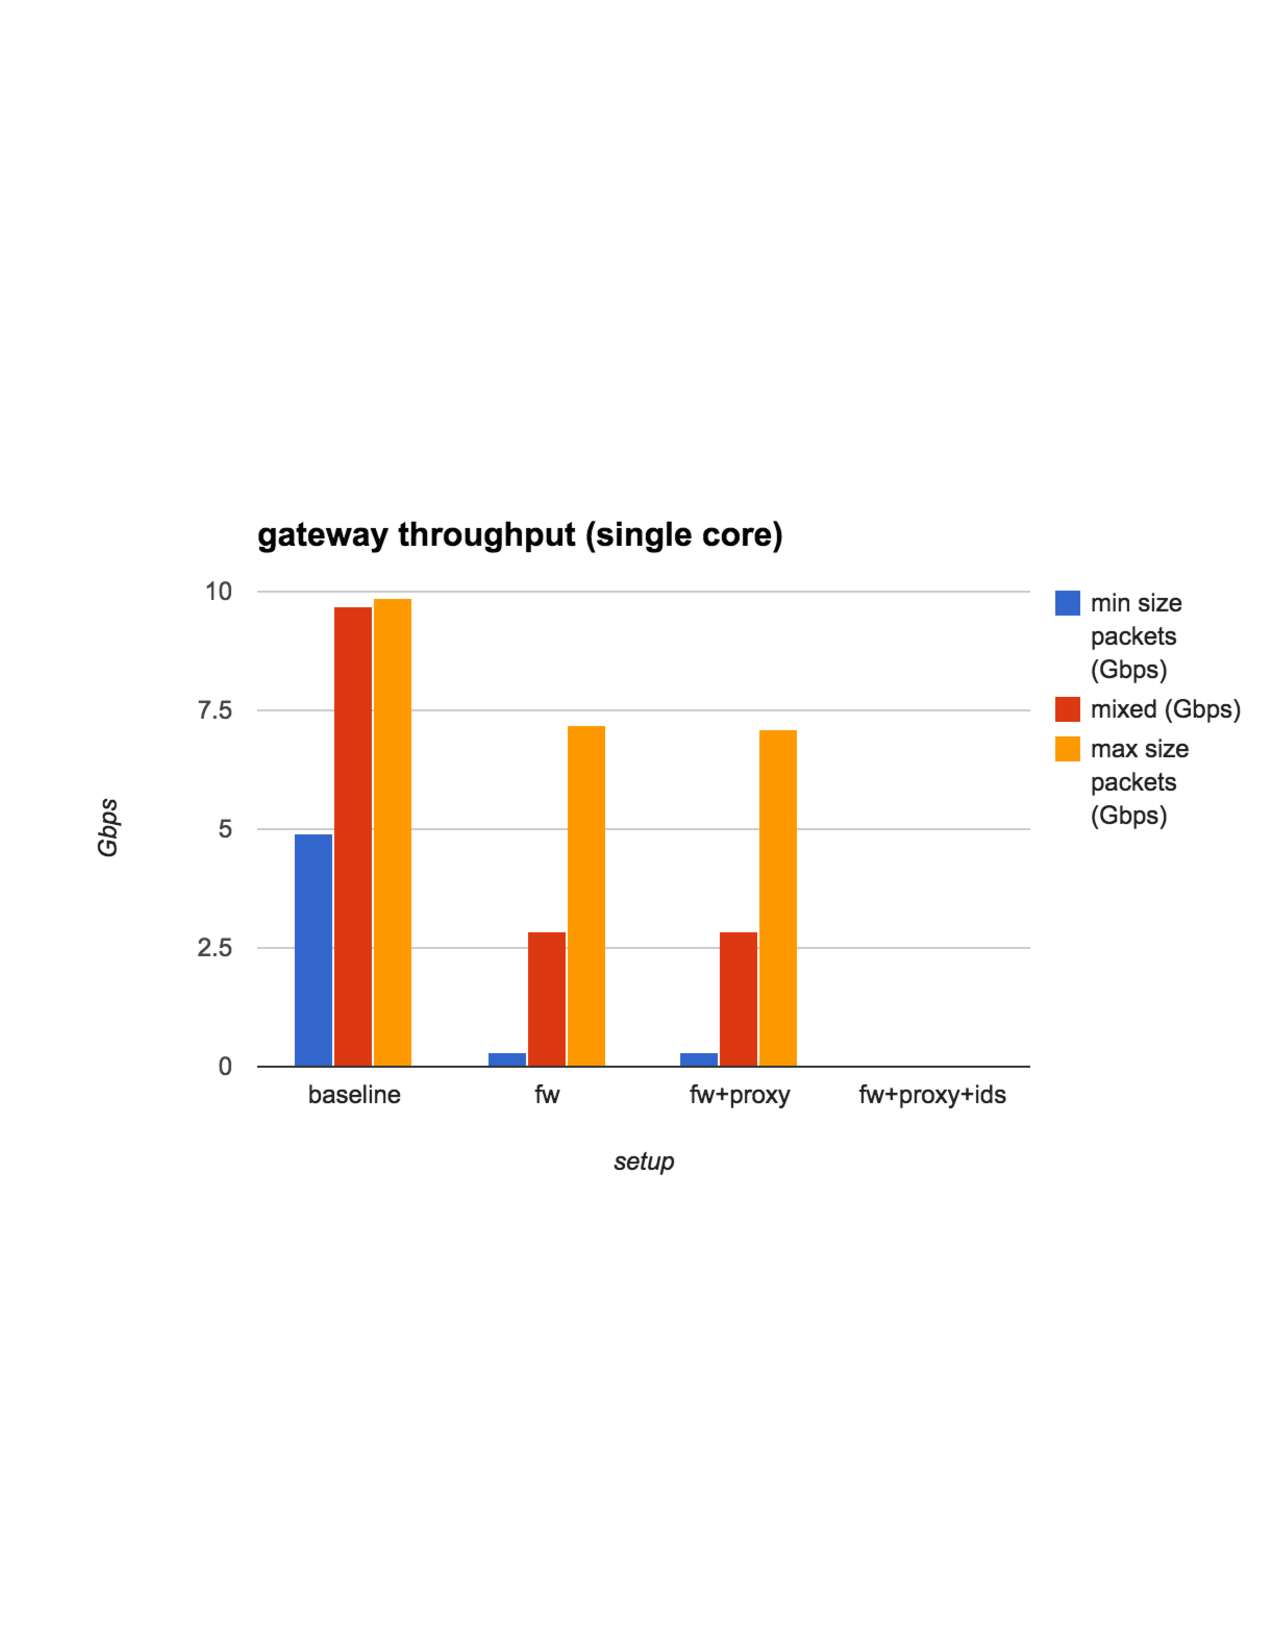
\includegraphics[height=1.25in]{fig/gatewayxput}&
  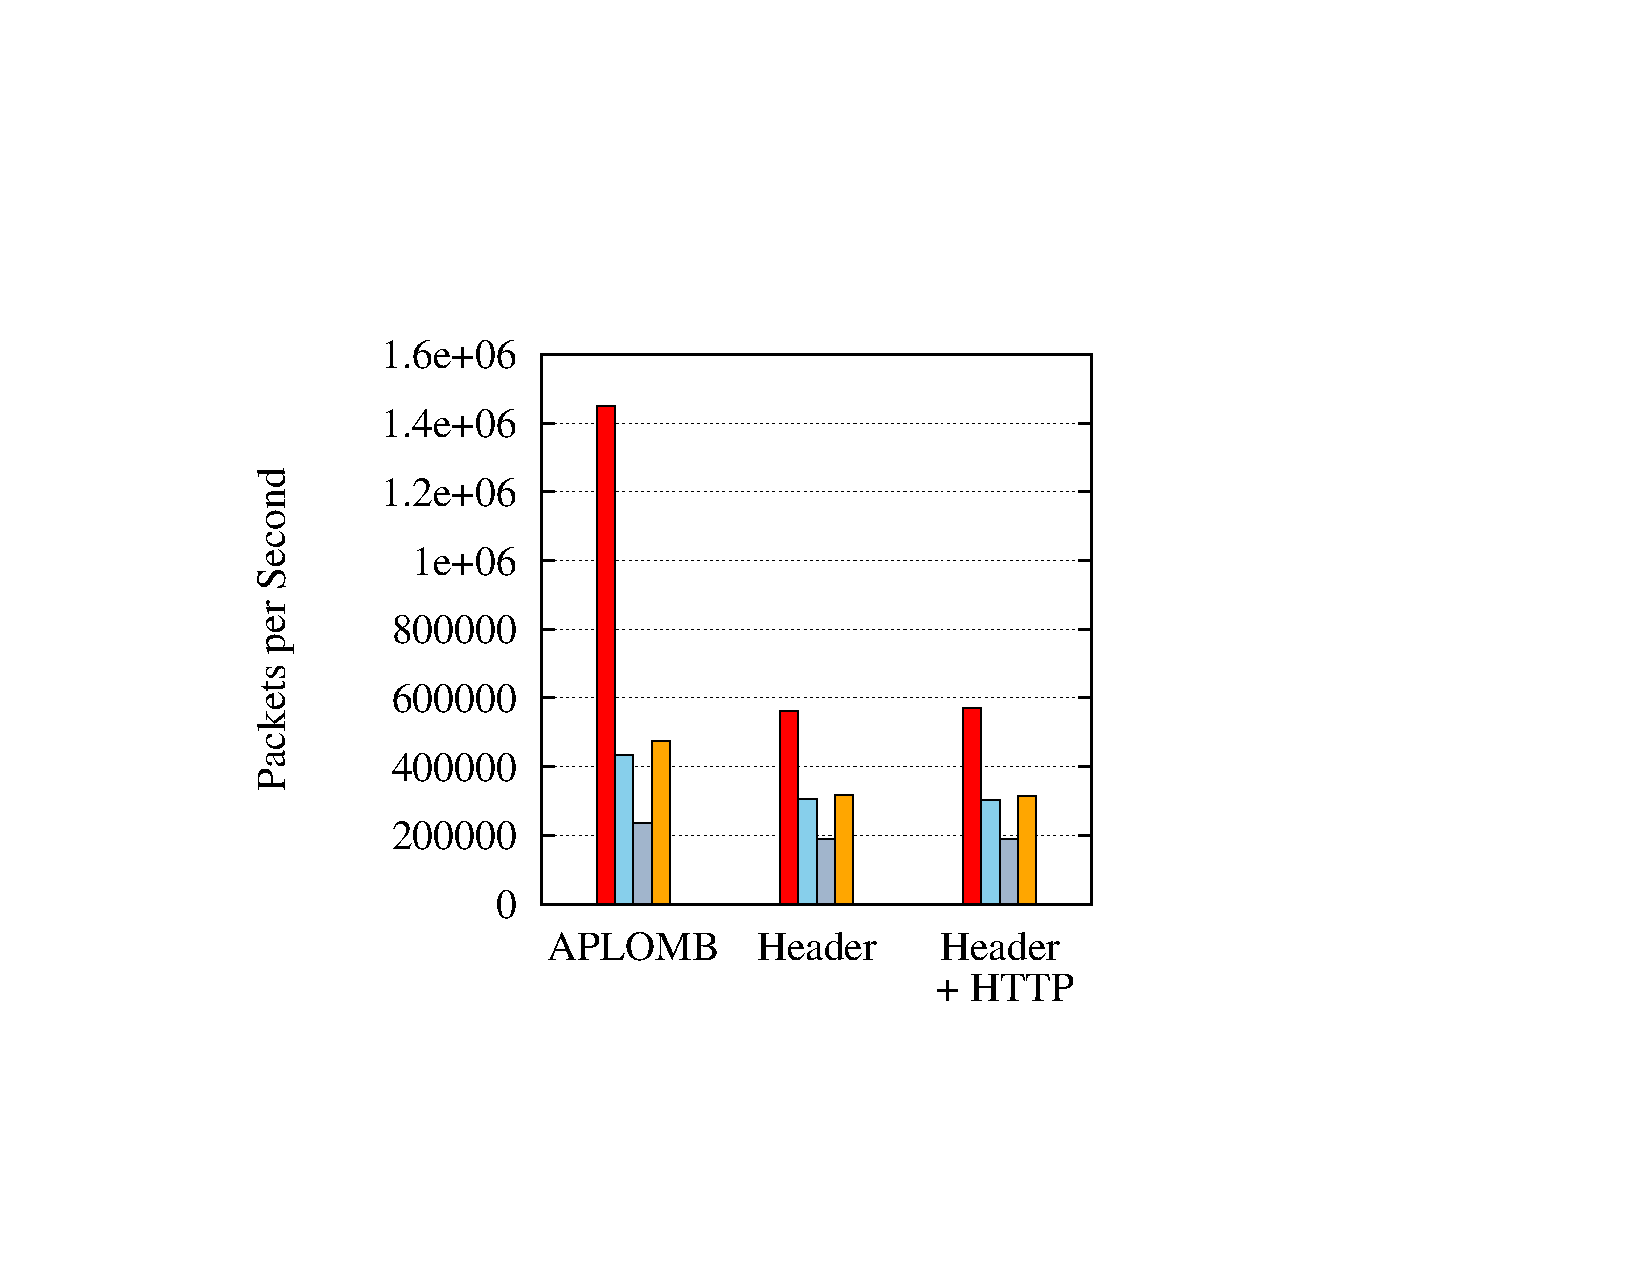
\includegraphics[height=1.25in]{fig/gateway_pps}\\
  \end{tabular}
  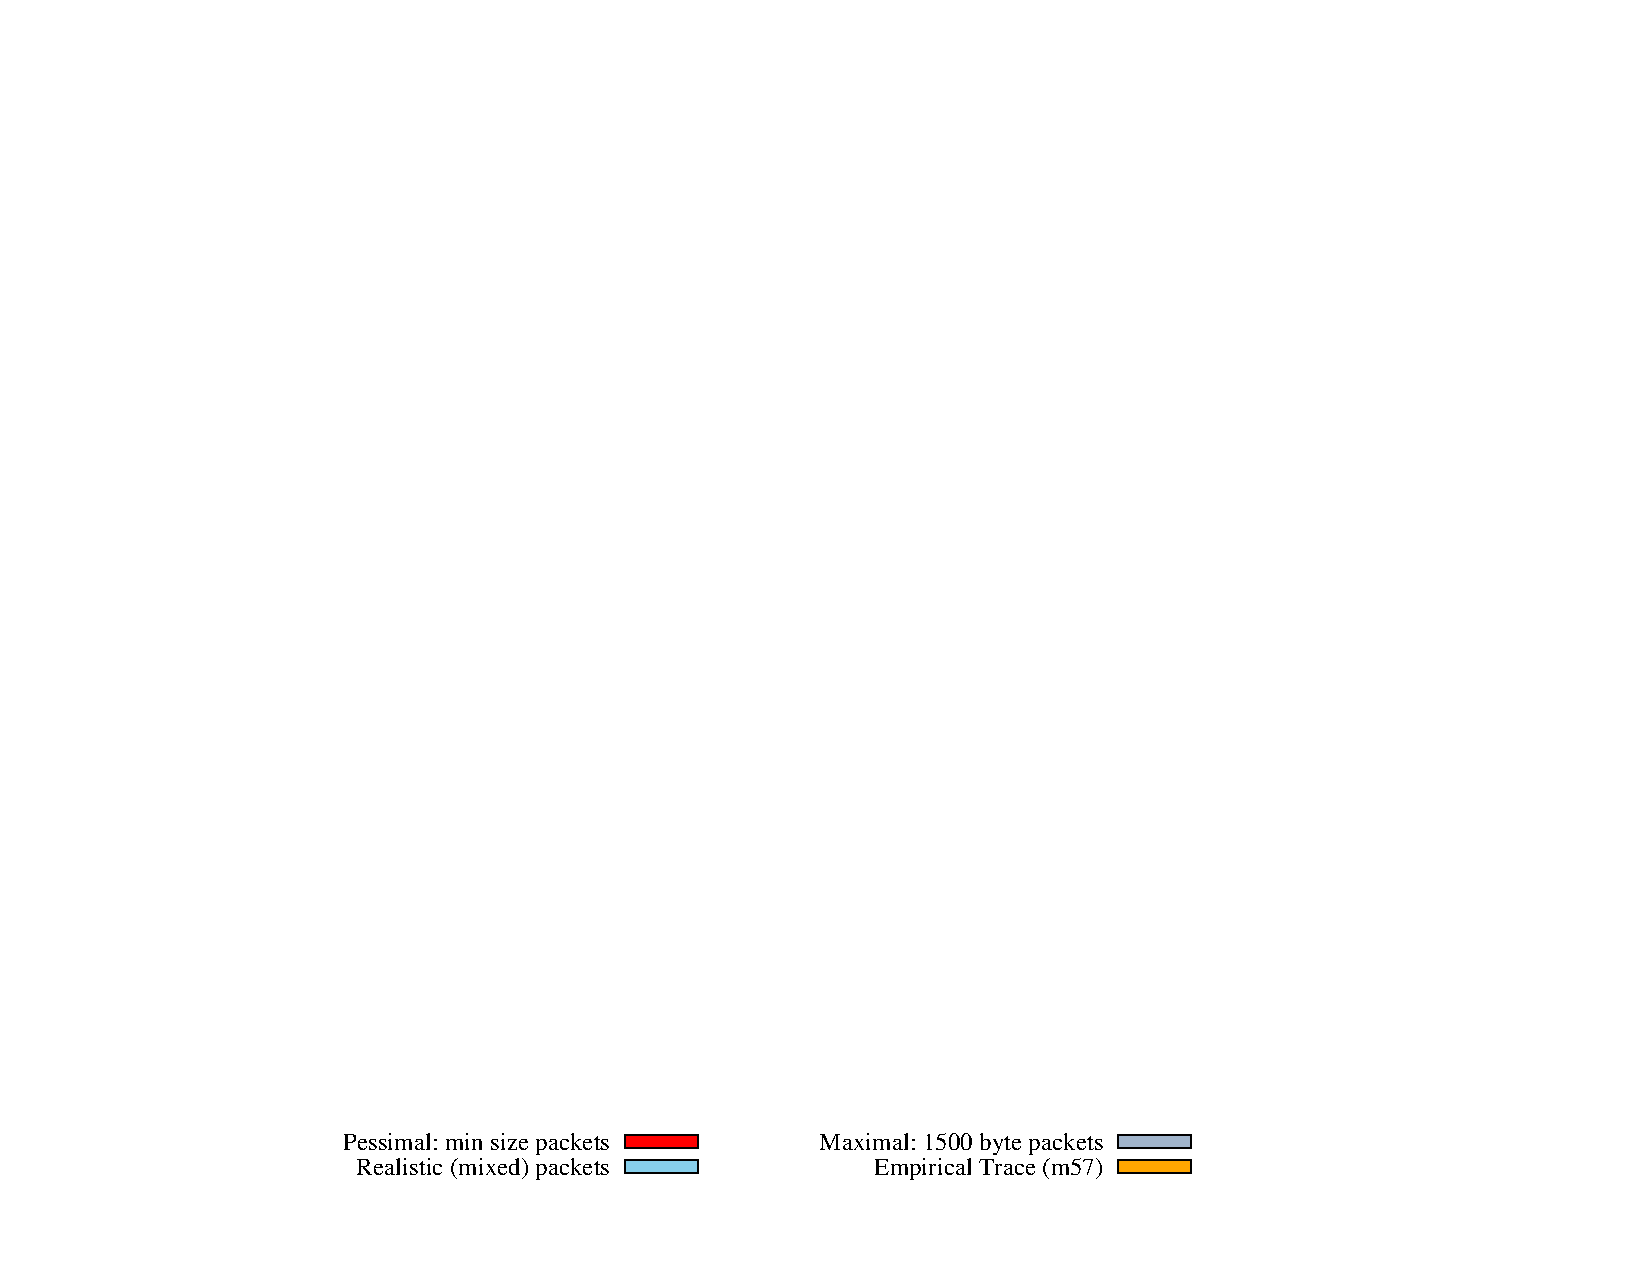
\includegraphics[width=2.75in]{fig/key}
  \caption[]{\label{fig:gwxput} Throughput/Packets per Second on a single core at the stateless gateway.}
\end{figure}

\noindent{\it How does encryption impact throughput at the outsourcing gateway?}
Figure~\ref{fig:gwxput} shows the gateway throughput when encrypting traffic to send to the cloud, first with normal redirection (as used in APLOMB~\cite{aplomb}), then with \sys's IP/TCP-header encryption, and finally with IP/TCP-header encryption as well as HTTP/proxy encryption. There is little difference between the HTTP overhead and the IP/TCP overhead, as the HTTP encryption only occurs on HTTP requests -- a small fraction of packets. Overall, \sys encryption for the stateless gateway reduces by about 60\% relative to baseline APLOMB encryption in the worst case (the min-sized workload; the reduction for the empirical (m57) workload is 38\%. Hence, an enterprise moving from a traditional outsourcing approach to \sys would need to provision at worst around 2.5$\times$ the number of processors at the outsourcing gateway.

\begin{figure}[t]
  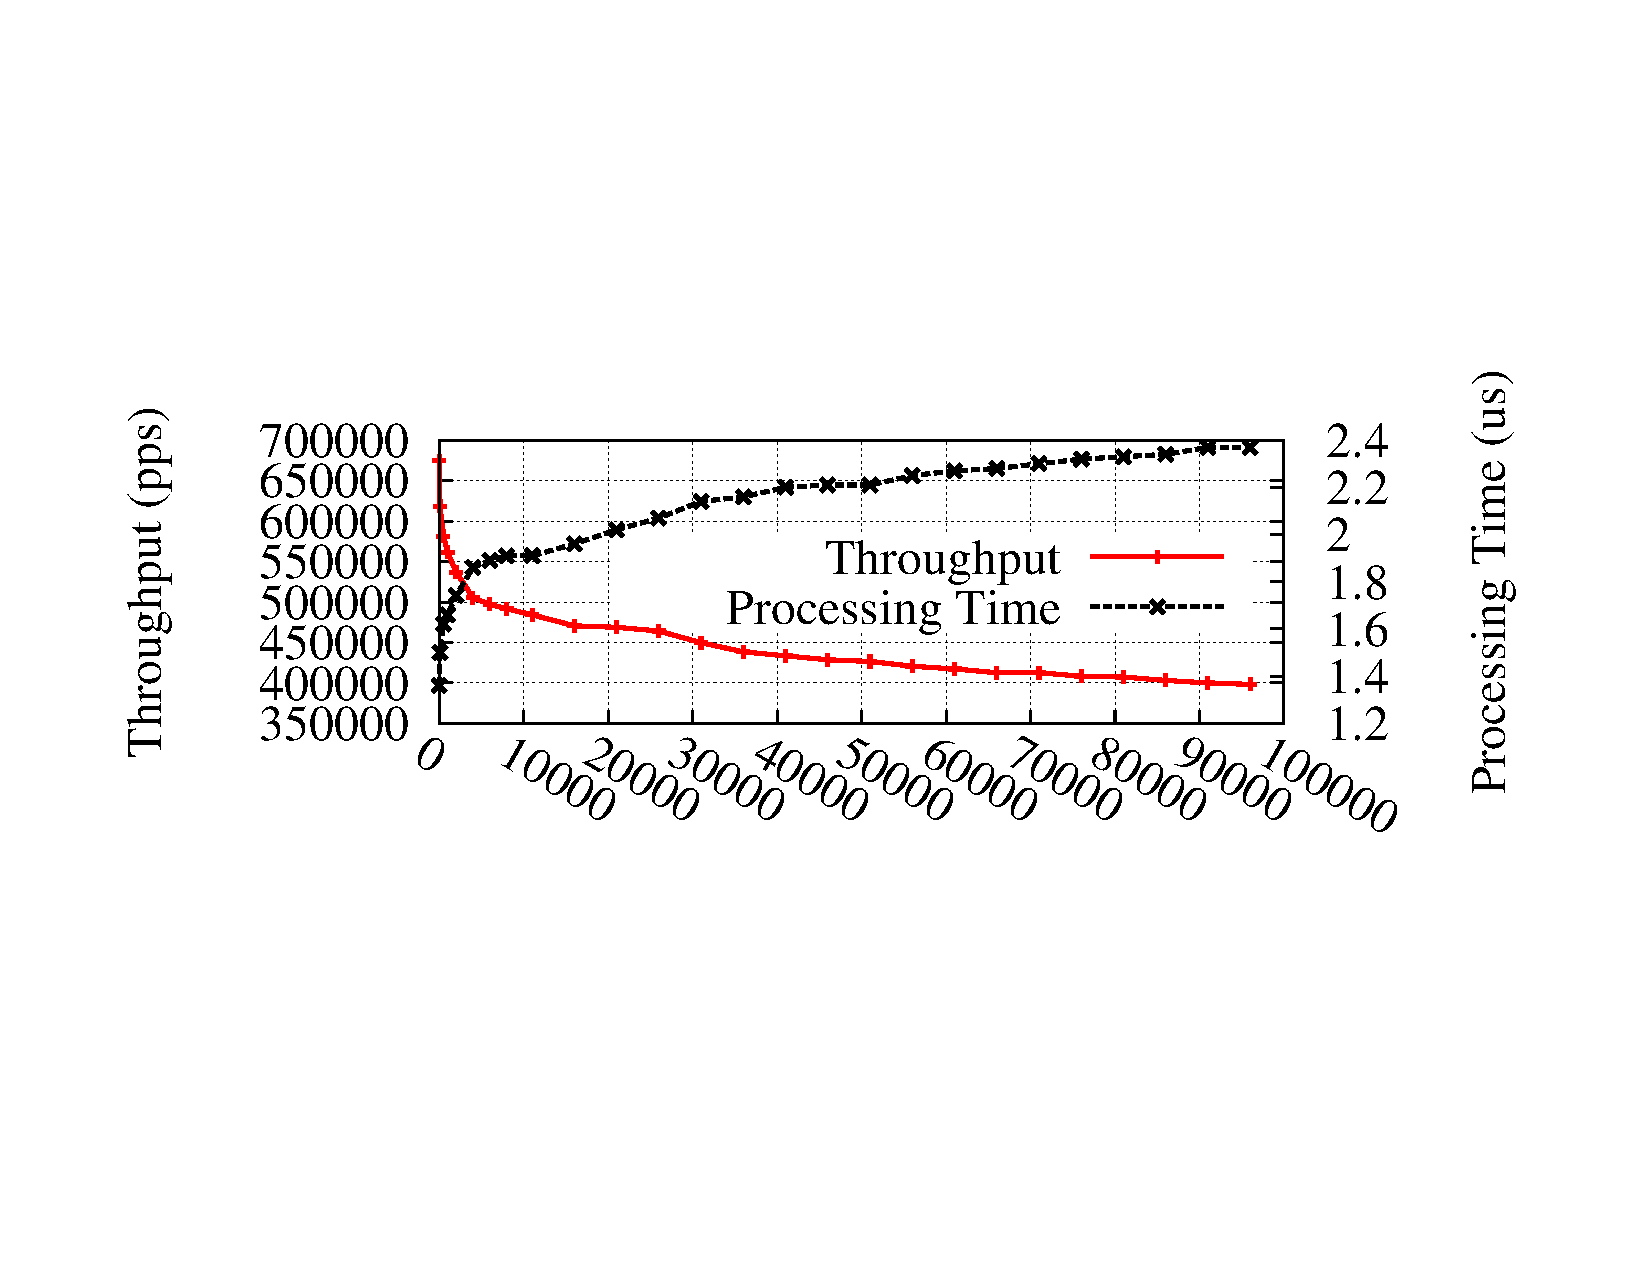
\includegraphics[width=3.25in]{fig/xputrange}
  \caption[]{\label{fig:xputrange} Throughput as number of rules for range encrypt increases.}
\end{figure}
\todo{call them rules or ranges? depending on the flow}

\noindent{\it How do throughput and latency at the gateway scale with the number of rules for range encryption?} 
In \S\ref{sec:range}, we discussed how our range encryption scheme stores encrypted values in a tree; every packet encryption requires a traversal of this tree.
Hence, as the size of the tree goes larger, we can expect to require more time to process each packet and throughput to decrease.
We measure this effect in Figure~\ref{fig:xputrange}. 
On the $y_1$ axis, we show the aggregate per packet throughput at the gateway as the number of rules from 0 to 100k. The penalty here is logarithmic, which is the expected performance of tree data structures. From 0-10k rules, throughput drops from 670Kpps to 480Kpps; after this point the performance penalty of additional rules tapers off. Adding an additional 90k rules drops throughput to 400Kpps.
On the $y_2$ axis, we measure the processing time per packet, \ie{}, the amount of time from when the gateway begins encrypting the packet to when the gateway completes encrypting the packet; the processing time follows the same logarithmic trend.
\todo{new latency numbers}

\noindent{\it Is range encryption faster than existing order preserving algorithms?}
Our range encryption is the only encryption scheme that has low enough latency for packet processing while preserving the ordering information needed for firewall rules. 
Existing order-preserving approaches require multiple round trip times -- and hence many milliseconds -- for each encryption operation.
Our range encoding approach encrypts each value in microseconds.
We compare against BCLO~\cite{boldyreva:ope} and mOPE~\cite{popa:mope} below:

\begin{table}[h]
\centering
\begin{tabular}{c|c|c|c}
Operation&BCLO~\cite{boldyreva:ope}&mOPE~\cite{popa:mope}&\sys\\
\hline
\hline
Encrypt, 10K rules&9333$\mu$s&6640$\mu$s&1,95$\mu$s\\
\hline
Encrypt, 100K rules&9333$\mu$s&8300$\mu$s&3$\mu$s\\
\hline
Decrypt&169$\mu$s&0.128$\mu$s&0.128$\mu$s\\
\hline
\end{tabular}
\end{table}

\noindent{\it What is the memory overhead of the stateful range map encryption scheme?}
Storing 10k rules in memory requires 1.6MB, and storing 100k rules in memory requires 28.5MB -- using unoptimized C++ objects.
This state overhead is negligible on any modern server.

\subsubsection{Header-Only Middleboxes}

\begin{table}[t!]
\begin{tabular}{p{3cm}|p{2cm}|p{2cm}}
Application &  Baseline Throughput & \sys Throughput \\
\hline \hline
IP Firewall &     &  \\
Application Firewall  & & \\
NAT &   &   \\
IP Forwarding  & & \\
%VPN Gateway &  &  &  \\ 
Load Balancer L4  & & \\
%Load Balancer L7 & & & \\
%WAN optimizer  & & & \\
Web Proxy & &\\
%IDS & & & \\
%Exfiltration/parental filtering & & &  \\
\end{tabular}
\caption{Middlebox applications supported by Header-Only \sys; throughput measured with an empirical traffic workload. \label{tbl:appsxput}}
\
\end{table}

\noindent{\it Is throughput reduced at the middleboxes due to Header-Only \sys?}
Table~\ref{tbl:appsxput}...\todo{FILL IN}



\noindent{\bf Firewalls.} 
{\it Does \sys support all rules in a typical firewall configuration? How much does the ruleset ``expand'' due to encryption?}

\noindent{\it How often do updates to the firewall require a rule refresh? How long does it take to refresh rules at the firewall?}

\noindent{\bf NAT.}
\noindent{\bf LB...}

\noindent{\bf Proxy/Caching.}
{\it How many active connections per second can the Proxy accept? How does this compare to an unencrypted Proxy implementation, like Squid?}

{\it What improvement in page load times does a client experience due to proxying, relative to no proxy at all? Relative to an unencrypted proxy implementation?}



\subsection{\sys with Bytestream Reconstruction}
In \S\ref{sec:something}, we discussed how the \sys gateway must be stateful to support bytestream-aware applications in order to encrypt end-to-end payloads properly for intrusion detection, and in order to parse the HTTP header for proxying pipelined HTTP connections. 
The overhead introduced by the bytestream-aware gateway is twofold: (1) the cost of stateful connection-keeping, and (2) the increased encryption cost, as cryptographic operations are performed over the payload (as much as 1500 bytes) rather than the headers (<30 bytes).
We tested the stateful proxy using an empirical workload of web page requests from the Alexa~\cite{alexa} top sites; on a single core the stateful gateway could forward at most 240Mbps -- about one-sixth the throughput of the stateless gateway over an empirical trace. 

We now evaluate the performance of our two bytestream-aware middleboxes: a proxy for pipelined connections, and an IDS.

\noindent{\bf Intrusion Detection}
Our IDS is based on BlindBox~\cite{blindbox}. However, \sys affords better performance and stronger privacy than BlindBox. BlindBox incurs a substantial `setup cost' every time a client initiates a new connection. With \sys, however, the gateway and the cloud maintain one, long-term persistent connection. 
Hence, this setup cost is paid once when the gateway is initially configured. This results in two benefits:

\noindent{\it (1) End-to-end performance improves.} Where BlindBox incurs an initial handshake of 414s~\cite{blindbox} to open a new connection, clients under \sys never pay this cost; instead they perform a normal TCP or SSL handshake of only 3-5 RTTs. In our testbed, this amounts to between 30 and 100 ms, depending on the site and protocol -- an improvement of 4 orders of magnitude.

\noindent{\it (2) Security improves.} As we presented in \S\ref{sec:ids}, BlindBox operates at one of two security levels: a stronger security level for exact-match strings, and a weaker security level for regular expressions. The stronger security level requires a round of handshake for each rule, but the weaker security level does not require more handshakes for each regular expression. 
With \sys, the initial handshake/setup is performed exactly once, between the gateway and the middlebox. 
Hence, we can convert regular expressions to exact match strings, even if they result in many hundreds of times more exact match rules. 
Consequently, more rules can be detected using the stronger security guarantee, without incurring any handshake overhead.
Using IDS rulesets from Snort, we converted regular expressions to exact match strings as discussed in \S\ref{sec:ids}; we were able to convert about half of all regular expressions to a finite number of exact match strings. 
Consequently, \sys can detect more then 80-88\% of attacks using the higher security level, rather than 42-67\% as with BlindBox:

\begin{table}[h]
  \centering
  \begin{tabular}{l|c|c}
    {\bf Dataset}&{\bf Exact Match}&{\bf Prob. Cause}\\
    \hline
    \hline
    BlindBox: Community&67\%&100\%\\
    \hline
    \sys: Community&88.7\%&100\%\\

    \hline
    \hline
    BlindBox: Emerging Threats&42\%&100\%\\
    \hline
    \sys: Emerging Threats&79.8\%&100\%\\
    \hline
  \end{tabular}
\end{table}

\noindent{\bf Proxy.} \todo{Can we say something here so it doesn't sound like we have a special gateway just for IDS? Because we do need this for IDS -- maybe, how much improvement over the non-pipeline proxy do we get?}



%!TEX root = mb.tex

\section{Related work}\label{sec:related}



Confidentiality of data in the cloud has been widely recognized as an important problem and researchers proposed solutions for generic applications~\cite{Baumann:Haven}, web applications \cite{giffin:hails, Mylar},  filesystems~\cite{blaze:cfs, kallahalla:plutus, goh:sirius},  databases~\cite{popa:cryptdb},  and virtual machines~\cite{Zhang:CloudVisor}. However, there has been almost no work on data confidentiality for network processing in the cloud. 
%\sys is the first system that enables running a wide range of middleboxes at the cloud while protecting the confidentiality of the traffic from the cloud.  

A few systems~\cite{Vern:Anonymize03, Vern:Anonymize06} attempt to anonymize the packet stream in the hope of hiding the identity of the hosts.
Unlike \sys, this approach breaks certain middlebox functionality and does not hide the data content.
Yamada et al.~\cite{Yamada_IDS} show how one can perform some limited processing on an 
SSL-encrypted packet.
     by using only the size of the data and the timing of packets. While this provides privacy, it does not 
     support middlebox processing. 


As discussed, computing on encrypted data promises to provide both confidentiality and functionality. Theoretical cryptographers developed fully homomorphic encryption~\cite{gentry:fhe, gentry:fhe-aes-eprint} and functional encryption~\cite{BSW11}, two schemes which can run any function over encrypted data. Unfortunately, these schemes remain prohibitively impractical by orders of magnitude~\cite{gentry:fhe-aes-eprint}.

The CryptDB~\cite{popa:cryptdb} system introduced a vision for building practical systems that compute on encrypted data, by using an efficient encryption scheme for each core operation in the system; \sys follows the same  vision. Unfortunately, none of the encryption schemes nor the systems techniques in CryptDB apply to our setting.  The order-preserving encryption~\cite{boldyreva:ope} used in CryptDB is 
 $>3000$ times slower than RangeMatch (\S\ref{sec:eval}) and cannot sustain realistic network throughputs; moreover, it leaks the order of the IP addresses encrypted, while RangeMatch protects this information. Similarly, we use KeywordMatch for equality checks which is more secure than CryptDB's deterministic encryption.% because it is randomized. %Finally, the database techniques in CryptDB do not apply to our networking setting. 

The BlindBox~\cite{blindbox} system enables running an IDS on encrypted traffic. Our IDS is built on top of BlindBox, but it is much more efficient and more secure than BlindBox as discussed in \S\ref{sec:ids} and \S\ref{sec:eval}. Moreover, BlindBox focuses only on DPI and IDS and does not provide solutions for other middleboxes. %such as firewall, NAT, load balancer, web proxy and others;  \sys supports these with new techniques. %In addition, \sys takes an overall systems view and integrates all the different middleboxes into a system architecture that can process encrypted traffic in the cloud in a multitude of ways.

%Moreover, \sys takes an overall systems view and develops a system architecture that can run a multitude of middleboxes  on encrypted traffic in the cloud.



Let us now present related work to our RangeMatch scheme. 
As  mentioned, order-preserving encryption  (OPE) schemes \cite{boldyreva:ope}, \cite{popa:mope} is less secure than RangeMatch because they leak order, and are $>3000$ slower than RangeMatch, which is not feasible for networks.
The  encryption scheme of Boneh et al.~\cite{BonehRange} enables detecting if an encrypted value matches a range and provides a similar security to ours. 
This scheme is less efficient, orders of magnitude more than OPE itself, its ciphertext size is exponential in the size of the input, and it does not support the ``>'' operator, which is the basis of fast matching algorithms at the firewall. By taking advantage of the networks and systems setting, we constructed  a much more efficient scheme. 
%  mOPE unfortunately requires that the gateway and the service provider interact for a number of roundtrips (e.g., xxx in our experiments) which is too slow and requires additional setup for this interaction, and violates requirement~\ref{req:sec} or~\ref{req:injective}, and BCLO has weak security (leaking always the top half bits of the values encrypted and the order of IP addresses across different packets, thus violating requirement~\ref{req:sec}), is too slow, and not format-preserving. 

% HERE ARE A FEW USEFUL NOTES ABOUT HOW OUR DESIGN IS DIFFERENT FROM mOPE -- THERE IS SOME SIMILARITY DUE TO TREE AND ADJUST
% we do not readjust for encryption 
% - this is expensive, we do not leak data between two encryptions 
% The tree is stored at the gateway. The tree contains as nodes the ends of the intervals as opposed to all values encoded-- thus, the tree is much smaller. firewalls have on the order of thousands such rules, so the tree is not large. also store only ranges and not everything encoded, making it smaller and fit into the gateway, etc., they need adjustments when they encrypt too, etc. -- better point to related work for this
% Difference:
% we encode different values in the tree, have a different encryption algorithm, and create a much smaller tree that can be stored at the gateway. no roundtrips any more; they don't have the deterministic property
%store the tree at the gateway.
% This tree is stored at the gateway. The tree stores edges of the interval 
% one important point is that there are ciphertext updates only for rule changes and not for regular encryption









%!TEX root = mb.tex

\section{Conclusions} \label{sec:concl}



In this paper, we presented \sys, the first system that enables running a wide range of middleboxes at a service provider 
while maintaining the confidentiality of traffic. \sys works by enabling the service provider to compute on the encrypted traffic without decrypting it. 
We showed that \sys supports a wide-range of middleboxes (such as firewall, NAT, web proxy, load balancing, IP forwarding, intrusion prevention systems, data exfiltration systems, and VPN), and provides competitive performance.  



%
% The following two commands are all you need in the
% initial runs of your .tex file to
% produce the bibliography for the citations in your paper.
\bibliographystyle{abbrv}
    \bibliography{related_work,cryptobib,rp,rp-str,rp-conf}
  % sigproc.bib is the name of the Bibliography in this case
% You must have a proper ".bib" file
%  and remember to run:
% latex bibtex latex latex
% to resolve all references




%
% ACM needs 'a single self-contained file'!
%
%APPENDICES are optional
\balancecolumns

% That's all folks!
\end{document}
